% Template adapted from https://github.com/jgm/pandoc-templates/blob/master/default.latex
% To be used with XeLaTex in memoiR
%%%%%%%%%%%%%%%%%%%%%%%%%%%%%%%%%%%%%%%%%%%%%%%%%%%%%%%%%%%%%%%%%%%%%%%%%%%%%%%%%%%%%%%%%

% Options for packages loaded elsewhere
\PassOptionsToPackage{unicode=true}{hyperref}
\PassOptionsToPackage{hyphens}{url}
\PassOptionsToPackage{dvipsnames,svgnames*,x11names*}{xcolor}
% Right to left support


\documentclass[
  11pt,
  american,
  a4paper,
  extrafontsizes,onecolumn,openright
  ]{memoir}

% Double (or whatever) spacing

% Math
\usepackage{amssymb, amsmath}
% mathspec: arbitrary math fonts
\usepackage{unicode-math}
\defaultfontfeatures{Scale=MatchLowercase}
\defaultfontfeatures[\rmfamily]{Ligatures=TeX,Scale=1}

% Fonts
\usepackage{lmodern}
\usepackage{fontspec}
% Main font
% Specific sanserif font
% Specific monotype font
% Specific math font
% Chinese, Japanese, Corean fonts

% Use upquote for straight quotes in verbatim environments
\usepackage{upquote}
% Use microtype
\usepackage[]{microtype}
\UseMicrotypeSet[protrusion]{basicmath} % disable protrusion for tt fonts

% Verbatim in note

% Color links
\usepackage{xcolor}

% Strikeout

% Necessary for code chunks
\usepackage{color}
\usepackage{fancyvrb}
\newcommand{\VerbBar}{|}
\newcommand{\VERB}{\Verb[commandchars=\\\{\}]}
\DefineVerbatimEnvironment{Highlighting}{Verbatim}{commandchars=\\\{\}}
% Add ',fontsize=\small' for more characters per line
\usepackage{framed}
\definecolor{shadecolor}{RGB}{248,248,248}
\newenvironment{Shaded}{\begin{snugshade}}{\end{snugshade}}
\newcommand{\AlertTok}[1]{\textcolor[rgb]{0.94,0.16,0.16}{#1}}
\newcommand{\AnnotationTok}[1]{\textcolor[rgb]{0.56,0.35,0.01}{\textbf{\textit{#1}}}}
\newcommand{\AttributeTok}[1]{\textcolor[rgb]{0.77,0.63,0.00}{#1}}
\newcommand{\BaseNTok}[1]{\textcolor[rgb]{0.00,0.00,0.81}{#1}}
\newcommand{\BuiltInTok}[1]{#1}
\newcommand{\CharTok}[1]{\textcolor[rgb]{0.31,0.60,0.02}{#1}}
\newcommand{\CommentTok}[1]{\textcolor[rgb]{0.56,0.35,0.01}{\textit{#1}}}
\newcommand{\CommentVarTok}[1]{\textcolor[rgb]{0.56,0.35,0.01}{\textbf{\textit{#1}}}}
\newcommand{\ConstantTok}[1]{\textcolor[rgb]{0.00,0.00,0.00}{#1}}
\newcommand{\ControlFlowTok}[1]{\textcolor[rgb]{0.13,0.29,0.53}{\textbf{#1}}}
\newcommand{\DataTypeTok}[1]{\textcolor[rgb]{0.13,0.29,0.53}{#1}}
\newcommand{\DecValTok}[1]{\textcolor[rgb]{0.00,0.00,0.81}{#1}}
\newcommand{\DocumentationTok}[1]{\textcolor[rgb]{0.56,0.35,0.01}{\textbf{\textit{#1}}}}
\newcommand{\ErrorTok}[1]{\textcolor[rgb]{0.64,0.00,0.00}{\textbf{#1}}}
\newcommand{\ExtensionTok}[1]{#1}
\newcommand{\FloatTok}[1]{\textcolor[rgb]{0.00,0.00,0.81}{#1}}
\newcommand{\FunctionTok}[1]{\textcolor[rgb]{0.00,0.00,0.00}{#1}}
\newcommand{\ImportTok}[1]{#1}
\newcommand{\InformationTok}[1]{\textcolor[rgb]{0.56,0.35,0.01}{\textbf{\textit{#1}}}}
\newcommand{\KeywordTok}[1]{\textcolor[rgb]{0.13,0.29,0.53}{\textbf{#1}}}
\newcommand{\NormalTok}[1]{#1}
\newcommand{\OperatorTok}[1]{\textcolor[rgb]{0.81,0.36,0.00}{\textbf{#1}}}
\newcommand{\OtherTok}[1]{\textcolor[rgb]{0.56,0.35,0.01}{#1}}
\newcommand{\PreprocessorTok}[1]{\textcolor[rgb]{0.56,0.35,0.01}{\textit{#1}}}
\newcommand{\RegionMarkerTok}[1]{#1}
\newcommand{\SpecialCharTok}[1]{\textcolor[rgb]{0.00,0.00,0.00}{#1}}
\newcommand{\SpecialStringTok}[1]{\textcolor[rgb]{0.31,0.60,0.02}{#1}}
\newcommand{\StringTok}[1]{\textcolor[rgb]{0.31,0.60,0.02}{#1}}
\newcommand{\VariableTok}[1]{\textcolor[rgb]{0.00,0.00,0.00}{#1}}
\newcommand{\VerbatimStringTok}[1]{\textcolor[rgb]{0.31,0.60,0.02}{#1}}
\newcommand{\WarningTok}[1]{\textcolor[rgb]{0.56,0.35,0.01}{\textbf{\textit{#1}}}}

% Listings package

% Tables
\usepackage{longtable,booktabs,tabu}
% Fix footnotes in tables (requires footnote package)
\IfFileExists{footnote.sty}{\usepackage{footnote}\makesavenoteenv{longtable}}{}

% Graphics
\usepackage{graphicx,grffile}
\graphicspath{{images/}}
\makeatletter
\def\maxwidth{\ifdim\Gin@nat@width>\linewidth\linewidth\else\Gin@nat@width\fi}
\def\maxheight{\ifdim\Gin@nat@height>\textheight\textheight\else\Gin@nat@height\fi}
\makeatother
% Scale images if necessary, so that they will not overflow the page
% margins by default, and it is still possible to overwrite the defaults
% using explicit options in \includegraphics[width, height, ...]{}
\setkeys{Gin}{width=\maxwidth,height=\maxheight,keepaspectratio}

% Prevent overfull lines
\setlength{\emergencystretch}{3em}  
\providecommand{\tightlist}{%
  \setlength{\itemsep}{0pt}\setlength{\parskip}{0pt}}

% Number sections for memoir (secnumdepth counter is ignored)
\setsecnumdepth{section}

% Set default figure placement to htbp
\makeatletter
\def\fps@figure{htbp}
\makeatother

% Spacing in lists
\usepackage{enumitem}

% Polyglossia
\usepackage{polyglossia}
\setmainlanguage{en-US}
\setotherlanguage{fr-FR}

% localized quotes
\usepackage[strict,autostyle]{csquotes}

% BibLaTeX
\usepackage[backend=biber,style=verbose-inote,pageref=true,isbn=false,backref=true,giveninits=true,uniquename=init,maxcitenames=2,maxbibnames=150,sorting=nyt,sortcites=false]{biblatex}
\addbibresource{references.bib}

% cslreferences environment required by pandoc > 2.7



%%%%%%%%%%%%%%%%%%%%%%%%%%%%%%%%%%%%%%%%%%%%%%%%%%%%%%%%%%
% memoiR format

% Chapter Summary environment 
\usepackage[tikz]{bclogo}
\newenvironment{Summary}
  {\begin{bclogo}[logo=\bctrombone, noborder=true, couleur=lightgray!50]{L'essentiel}\parindent0pt}
  {\end{bclogo}}
% Syntax:
%
%```{block, type='Summary'}
% Deliver message here.
% ```

% scriptsize code 
\let\oldverbatim\verbatim
\def\verbatim{\oldverbatim\scriptsize}
% Applies to code blocks and R code results
% code chunk options size='scriptsize' applies only to R code and results
% if the code chunk sets a different size, \def\verbatim{...} is prioritary for code results 


% memoiR dalef3 chapter style 
% https://ctan.crest.fr/tex-archive/info/latex-samples/MemoirChapStyles/MemoirChapStyles.pdf
\usepackage{soul}
\definecolor{nicered}{rgb}{.647,.129,.149}
\makeatletter
\newlength\dlf@normtxtw
\setlength\dlf@normtxtw{\textwidth}
\def\myhelvetfont{\def\sfdefault{mdput}}
\newsavebox{\feline@chapter}
\newcommand\feline@chapter@marker[1][4cm]{%
  \sbox\feline@chapter{%
    \resizebox{!}{#1}{\fboxsep=1pt%
	  \colorbox{nicered}{\color{white}\bfseries\sffamily\thechapter}%
	}}%
  \rotatebox{90}{%
    \resizebox{%
	  \heightof{\usebox{\feline@chapter}}+\depthof{\usebox{\feline@chapter}}}%
	{!}{\scshape\so\@chapapp}}\quad%
  \raisebox{\depthof{\usebox{\feline@chapter}}}{\usebox{\feline@chapter}}%
 }
\newcommand\feline@chm[1][4cm]{%
  \sbox\feline@chapter{\feline@chapter@marker[#1]}%
  \makebox[0pt][l]{% aka \rlap
    \makebox[1cm][r]{\usebox\feline@chapter}%
  }}
\makechapterstyle{daleif1}{
  \renewcommand\chapnamefont{\normalfont\Large\scshape\raggedleft\so}
  \renewcommand\chaptitlefont{\normalfont\huge\bfseries\scshape\color{nicered}}
  \renewcommand\chapternamenum{}
  \renewcommand\printchaptername{}
  \renewcommand\printchapternum{\null\hfill\feline@chm[2.5cm]\par}
  \renewcommand\afterchapternum{\par\vskip\midchapskip}
  \renewcommand\printchaptertitle[1]{\chaptitlefont\raggedleft ##1\par}
}
\makeatother


% Layout
%%%%%%%%%%%%%%%%%%%%%%%%%%%%%%%%%%%%%%%%%%%%%%%%%%%%%%%%%%

% Based on memoir, style companion
\newcommand{\MemoirChapStyle}{companion}
\newcommand{\MemoirPageStyle}{companion}

% Space between paragraphs
\usepackage{parskip}
  \abnormalparskip{3pt}

% Adjust margin paragraphs vertical position
\usepackage{marginfix}


% Margins
%%%%%%%%%%%%%%%%%%%%%%%%%%%%%%%%%%%%%%%

% allow use of '-',+','/' ans '*' to make simple length computation
\usepackage{calc}

% Full-width figures utilities
\newlength\widthw % full width
\newlength{\rf}
\newcommand*{\definesHSpace}{
  \strictpagecheck % slower but efficient detection of odd/even pages
  \checkoddpage
  \ifoddpage
  \setlength{\rf}{0mm}
  \else
  \setlength{\rf}{\marginparsep+\marginparwidth}
  \fi
}

\makeatletter
% 1" margins for the front matter.
\newcommand*{\SmallMargins}{
  \setlrmarginsandblock{1.2in}{1.5in}{*}
  \setmarginnotes{0.1in}{0.1in}{0.1in}
 \setulmarginsandblock{1.5in}{1in}{*}
  \checkandfixthelayout
  \ch@ngetext
  \clearpage
  \setlength{\widthw}{\textwidth+\marginparsep+\marginparwidth}
  \footnotesatfoot
  \chapterstyle{\MemoirChapStyle}  % Chapter and page styles must be recalled
  \pagestyle{\MemoirPageStyle}
}

% 3" outer margin for the main matter
\newcommand*{\LargeMargins}{
  \setlrmarginsandblock{1.2in}{3in}{*}
  \setmarginnotes{0.2in}{1.8in}{0.1in}
  \setsidecaps{0.2in}{1.8in}
  \setulmarginsandblock{1.5in}{1in}{*}
  \checkandfixthelayout
  \ch@ngetext
  \clearpage
  \setlength{\widthw}{\textwidth+\marginparsep+\marginparwidth}
  \footnotesinmargin
  \chapterstyle{\MemoirChapStyle}  % Chapter and page styles must be recalled
  \pagestyle{\MemoirPageStyle}
}
\makeatother

% Figure captions and footnotes in outer margins
\usepackage[margincaption,outercaption,ragged,wide]{sidecap}


% Local toc
%%%%%%%%%%%%%%%%%%%%%%%%%%%%%%%%%%%%%%%%%%%%%%%%%%%%%%%%%%

\usepackage{titletoc}
\newcommand{\toc}[1]{%
  \startcontents[chapters]%
  \printcontents[chapters]{}{1}[#1]{}%
  ~\newline%
}


% Text boxes
%%%%%%%%%%%%%%%%%%%%%%%%%%%%%%%%%%%%%%%%%%%%%%%%%%%%%%%%%%

% Define a style for mdframed boxes
\mdfdefinestyle{boxstyle}{
	skipabove=1.5\topskip,
	skipbelow=.5\topskip,
	rightmargin=0pt,
	leftmargin=0pt,
	innerrightmargin=7pt,
	innerleftmargin=7pt,
	topline=false,
	bottomline=false,
	rightline=false,
	leftline=false,
	frametitlerule=true,
	linecolor=black,
	fontcolor=black,
	frametitlealignment=\noindent
}


% Main title page with filigrane
%%%%%%%%%%%%%%%%%%%%%%%%%%%%%%%%%%%%%%%%%%%%%%%%%%%%%%%%%%

% Text blocks
\usepackage[absolute,overlay]{textpos}
  \setlength{\TPHorizModule}{1mm}
  \setlength{\TPVertModule}{1mm}

\newcommand{\MainTitlePage}[2]{
  \SmallMargins % Margins
  \pagestyle{empty} % No header/footer
  \textblockorigin{\stockwidth-\paperwidth-\trimedge}{\trimtop} % recto
  \begin{textblock*}{2mm}(\spinemargin/2,\uppermargin/2)
    \rule{1pt}{\paperheight-\uppermargin}
  \end{textblock*}
  \begin{textblock*}{\paperwidth*2/3}(\paperwidth/5, \paperheight/5)
    \flushright
    \begin{Spacing}{3}
      {\fontfamily{qtm}\selectfont\fontsize{45}{45}\selectfont\textsc{\thetitle}}
    \end{Spacing}
  \end{textblock*}
    \begin{textblock*}{\paperwidth/2}[1, 1](\paperwidth, \paperheight)
    \includegraphics[width=\paperwidth/2]{filigrane}
  \end{textblock*}
  \begin{textblock*}{\paperwidth*2/3}(\spinemargin, \paperheight/2)
    {\fontfamily{qtm}\huge\theauthor}
  \end{textblock*}
    \begin{textblock*}{\paperwidth*2/3}[0, 1](\spinemargin, \uppermargin+\textheight)
    \normalfont\thedate
  \end{textblock*}
  ~\\ % Print a character or the page will not exist
  \newpage
  \textblockorigin{\trimedge}{\trimtop} % verso
  \begin{textblock*}{\textwidth}(\paperwidth-\spinemargin-\textwidth, \uppermargin)
    #1
  \end{textblock*}
  \begin{textblock*}{\textwidth}[0,1](\paperwidth-\spinemargin-\textwidth, \uppermargin+\textheight+\footskip)
    \centering
        #2
  \end{textblock*}
  ~\\ % Print a character or the page will not exist
  \newpage
}

% Clear page and open an even one (\clearpage opens an odd one)
\newcommand{\evenpage}{
  \clearpage
  \strictpagecheck % slower but efficient detection of odd/even pages
  \checkoddpage
  \ifoddpage
    \thispagestyle{empty}
    ~\\ % Print a character or the page will not exist
    \newpage
  \else
    % do nothing
  \fi
}


%% PDF title page to insert
%%%%%%%%%%%%%%%%%%%%%%%%%%%%%%%%%%%%%%%%%%%%%%%%%%%%%%%%%%



%% Bibliography
%%%%%%%%%%%%%%%%%%%%%%%%%%%%%%%%%%%%%%%%%%%%%%%%%%%%%%%%%%

% Repeated citation as author-year-title instead of author-title (modification of footcite:note in verbose-inote.cbx)
\renewbibmacro*{footcite:note}{%
  \ifnameundef{labelname}
    {\printfield{label}}
    {\printnames{labelname}}
  \setunit*{\nameyeardelim}
  \iffieldundef{labelyear}
    {}
    {\printtext[parens]{\printfield{labelyear}\printfield{userb}}.}
  \ifsamepage{\the\value{instcount}}{\csuse{cbx@f@\thefield{entrykey}}}
    {}
    {\setunit*{\nametitledelim} \printfield[title]{labeltitle}}
  \setunit*{\addcomma\space}
  \printtext{
    \bibstring{seenote}\addnbspace
    \ref{cbx@\csuse{cbx@f@\thefield{entrykey}}}
    \iftoggle{cbx:pageref}
    {
      \ifsamepage{\the\value{instcount}}  {\csuse{cbx@f@\thefield{entrykey}}}
      {}
      {\addcomma\space\bibstring{page}\addnbspace
      \pageref{cbx@\csuse{cbx@f@\thefield{entrykey}}}
      }
    }
    {}
  }
}
% Normal text in citations, to allow \textcite
\AtEveryCite{\renewcommand*{\mkbibnamefamily}[1]{\textnormal{#1}}}
% Add url's to computer softfware and @Misc in general, delete it in other cases
% in citations...
\AtEveryCitekey{%
  \ifentrytype{misc}{%
  }{%
  \clearfield{url}%
  \clearfield{urldate}%
  }%
}
% ... and in bibliography
\AtEveryBibitem{%
  \ifentrytype{misc}{%
  }{%
  \clearfield{url}%
  \clearfield{urldate}%
}%
}

%% Table of Contents
%%%%%%%%%%%%%%%%%%%%%%%%%%%%%%%%%%%%%%%%%%%%%%%%%%%%%%%%%%

% fix the typesetting of the part number
\renewcommand\partnumberlinebox[2]{#2\ ---\ }


% Fonts
%%%%%%%%%%%%%%%%%%%%%%%%%%%%%%%%%%%%%%%%%%%%%%%%%%%%%%%%%%

% Font size of side captions and side notes
\captionnamefont{\scriptsize}
\captiontitlefont{\scriptsize}
\renewcommand{\footnotesize}{\tiny}

% Hyperref comes last
%%%%%%%%%%%%%%%%%%%%%%%%%%%%%%%%%%%%%%%%%%%%%%%%%%%%%%%%%%

\usepackage{hyperref}
\hypersetup{
  pdftitle={Mesures de la Biodiversité},
  pdfauthor={Eric Marcon},
  colorlinks=true,
  linkcolor=Maroon,
  citecolor=Blue,
  urlcolor=blue,
  breaklinks=true}

% Don't use monospace font for urls
\urlstyle{same}


% Title, author, date from YAML to LaTeX
%%%%%%%%%%%%%%%%%%%%%%%%%%%%%%%%%%%%%%%%%%%%%%%%%%%%%%%%%%

\title{Mesures de la Biodiversité}

\author{Eric Marcon}

\date{23/12/2023}


% Include headers (preamble.tex) here
%%%%%%%%%%%%%%%%%%%%%%%%%%%%%%%%%%%%%%%%%%%%%%%%%%%%%%%%%%
% Add LaTeX code into the preamble of the document here
\hyphenation{bio-di-ver-si-ty sap-lings}

% Define colors for text boxes
\definecolor{grey}{HTML}{F5F5F5}

% Define text box environments
\newmdenv[
	style=boxstyle,
	backgroundcolor=grey,
	frametitlebackgroundcolor=grey,
]{greybox}
\usepackage{booktabs}
\usepackage{longtable}
\usepackage{array}
\usepackage{multirow}
\usepackage{wrapfig}
\usepackage{float}
\usepackage{colortbl}
\usepackage{pdflscape}
\usepackage{tabu}
\usepackage{threeparttable}
\usepackage{threeparttablex}
\usepackage[normalem]{ulem}
\usepackage{makecell}
\usepackage{xcolor}


% End of preamble
%%%%%%%%%%%%%%%%%%%%%%%%%%%%%%%%%%%%%%%%%%%%%%%%%%%%%%%%%%


\begin{document}
\frontmatter

% Title page
%%%%%%%%%%%%%%%%%%%%%%%%%%%%%%%%%%%%%%%%%%%%%%%%%%%%%%%%%%


\MainTitlePage{Ce document est réalisé de façon dynamique et reproductible grâce à:

\begin{itemize}
  \item \LaTeX, dans sa distribution Miktex (\url{http://miktex.org/}) et la classe memoir (\url{http://www.ctan.org/pkg/memoir}).
  \item R (\url{http://www.r-project.org/}) et RStudio (\url{http://www.rstudio.com/})
  \item bookdown (\url{http://bookdown.org/})
\end{itemize}

Son code source est sur GitHub: \url{https://github.com/EricMarcon/MesuresBioDiv2/}.
Le texte mis à jour en continu peut être lu sur \url{https://ericmarcon.github.io/MesuresBioDiv2/}.
Les versions d'étape sont déposées sur HAL: \url{https://hal-agroparistech.archives-ouvertes.fr/cel-01205813/}.}{Photographie en couverture: Hadrien Lalagüe}


% Before Body
%%%%%%%%%%%%%%%%%%%%%%%%%%%%%%%%%%%%%%%%%%%%%%%%%%%%%%%%%%





% Contents
%%%%%%%%%%%%%%%%%%%%%%%%%%%%%%%%%%%%%%%%%%%%%%%%%%%%%%%%%%

\LargeMargins
{
\hypersetup{linkcolor=}
\setcounter{tocdepth}{2}
\tableofcontents
}


% Body
%%%%%%%%%%%%%%%%%%%%%%%%%%%%%%%%%%%%%%%%%%%%%%%%%%%%%%%%%%

\LargeMargins
\hypertarget{motivation}{%
\chapter*{Motivation}\label{motivation}}
\addcontentsline{toc}{chapter}{Motivation}

Le terme \emph{biodiversity} est attribué \autocite{Meine2006} à Walter Rosen, un membre du \emph{National Research Council} américain, qui a commencé à contracter les termes \emph{biological diversity} pendant la préparation d'un colloque dont les actes seront publiés sous le titre \enquote{Biodiversity} \autocite{Wilson1988}.
La question de la diversité biologique intéressait les écologues bien avant l'invention de la biodiversité, mais le néologisme a connu un succès fulgurant \autocite{Blandin2014} en même temps qu'il devenait une notion floue, dans lequel chacun peut placer ce qu'il souhaite y trouver, au point de lui retirer son caractère scientifique \autocite{Delord2014}.
Une cause de ce glissement est que la biodiversité a été nommée pour attirer l'attention sur son érosion, en lien avec la biologie de la conservation.
Cette érosion concernant potentiellement de nombreux aspects du monde vivant, la définition de la biodiversité fluctue selon les besoins: \textcite{DeLong1996} en recense 85 dans les dix premières années de littérature.
Les indicateurs de la biodiversité peuvent englober bien d'autres choses que la diversité du vivant: le nombre d'espèces menacées (par exemple la liste rouge de l'IUCN), la taille des populations ou la surface des écosystèmes préservés, la dégradation des habitats, la menace pesant sur des espèces emblématiques\ldots{}
Une mesure rigoureuse et cohérente de la diversité peut pourtant être construite pour clarifier beaucoup (mais pas tous) des concepts qui constituent la biodiversité.

Dans l'introduction du premier chapitre des actes de ce qui était devenu le \enquote{Forum sur la Biodiversité}, Wilson utilise le mot dans le sens étroit de nombres d'espèces.
L'élargissement de la notion aux \enquote{systèmes naturels} et à l'opposé à la diversité génétique intraspécifique est venu du monde de la conservation \autocite{Speth1992}.
La déclaration de Michel Loreau, président du du comité scientifique de la conférence de Paris en 2005 \autocite{Loreau2005} en donne une définition aboutie:

\begin{quote}
La Terre abrite une extraordinaire diversité biologique, qui inclut non seulement les espèces qui habitent notre planète, mais aussi la diversité de leurs gènes, la multitude des interactions écologiques entre elles et avec leur environnement physique, et la variété des écosystèmes complexes qu'elles constituent.
Cette biodiversité, qui est le produit de plus de 3 milliards d'années d'évolution, constitue un patrimoine naturel et une ressource vitale dont l'humanité dépend de multiples façons.
\end{quote}

Aujourd'hui encore, le terme \emph{biodiversité} concerne le plus souvent la richesse en espèces d'un écosystème.
Pour simplifier la présentation, le niveau d'étude dans ce document sera en général celui des espèces \autocite[autre concept flou,][]{Hey2001}.
La prise en compte de la totalité des êtres vivants est généralement hors de portée.
La mesure de diversité est alors limitée à un taxocène, c'est-à-dire un sous-ensemble des espèces d'une communauté reliées taxonomiquement: les papillons, les mammifères, les arbres (la délimitation du sous-ensemble n'est pas forcément strictement taxonomique)\ldots{}

Un objet privilégié des études sur la biodiversité est, depuis le Forum, la forêt tropicale parce qu'elle est très diverse et un enjeu pour la conservation.
La plupart des exemples concerneront ici les arbres de la forêt tropicale, qui ont l'avantage d'être clairement définis en tant qu'individus (donc simples à compter) et posent des problèmes méthodologiques considérables pour l'estimation de leur diversité à partir de données réelles.

On peut bien évidemment s'intéresser à d'autres niveaux et d'autres objets, par exemple la diversité génétique (en termes d'allèles différents pour certains gènes ou marqueurs) à l'intérieur d'une population, ou même la diversité des interactions entre espèces d'une communauté \autocite{Jizhong1991}.
On gardera toujours à l'esprit que la prise en compte de la diversité spécifique n'est pas la seule approche, les méthodes présentées ici s'appliquent à la mesure de la diversité en général, pas même nécessairement biologique.

L'objectif de ce document est de traiter la mesure de la biodiversité, pas son importance en tant que telle.
On se référera par exemple à \textcite{Chapin2000} pour une revue sur cette question, \textcite{Cardinale2012} pour les conséquences de l'érosion de la biodiversité sur les services écosystémiques ou \textcite{Ceballos2017} pour les propriétés autocatalytiques de la biodiversité.

La mesure de la diversité est un sujet important en tant que tel \autocite{Purvis2000}, pour permettre de formaliser les concepts et de les appliquer à la réalité.
La question est loin d'être épuisée, et fait toujours l'objet d'une recherche active et de controverses \autocite{Ricotta2005b}.

\hypertarget{calculs-et-donnuxe9es}{%
\chapter*{Calculs et données}\label{calculs-et-donnuxe9es}}
\addcontentsline{toc}{chapter}{Calculs et données}

La présentation des mesures de diversité est donnée avec un usage intensif du formalisme mathématique.
La liste des notations est fournie ci-dessous, on s'y référera autant que nécessaire.

Les calculs sont réalisés dans R \autocite{R}, essentiellement avec le package \emph{divent} \autocite{R-divent}, qui succède au package \emph{entropart} \autocite{Marcon2014c}.
L'ensemble du code est disponible sur GitHub\footnote{\url{https://github.com/EricMarcon/MesuresBioDiv3/}} où se trouvent les mises à jour de ce document\footnote{\url{https://ericmarcon.github.io/MesuresBioDiv3/}}.

Les données sont souvent celles de la parcelle 6 de la forêt de Paracou (figure \ref{fig:Paracou6MapFig} en Guyane française \autocite{Gourlet-Fleury2004}, d'une surface de 6.25~ha.
Tous les arbres de plus de 10~cm de diamètre à hauteur de poitrine (DBH: \emph{Diameter at Breast Height}) y ont été inventoriés en 2016.
La position de chaque arbre, son espèce et sa surface terrière sont fournis.

D'autres exemples utilisent la parcelle forestière permanente de Barro Colorado Island, souvent abrégée BCI \autocite{Condit2012}: 50~ha de forêt tropicale dont les arbres de plus de 1~cm de diamètre à hauteur de poitrine (DBH: \emph{Diameter at Breast Height}) ont été inventoriés.
Le jeu de données utilisé pour les exemples est une version réduite aux arbres de plus de 10~cm disponible dans le package \emph{vegan} \autocite{Oksanen2012}, soient 21457 arbres dans 225 espèces.



\scriptsize

\begin{figure}\setbox0=\hbox{\begin{minipage}[h]{\widthw}\centering 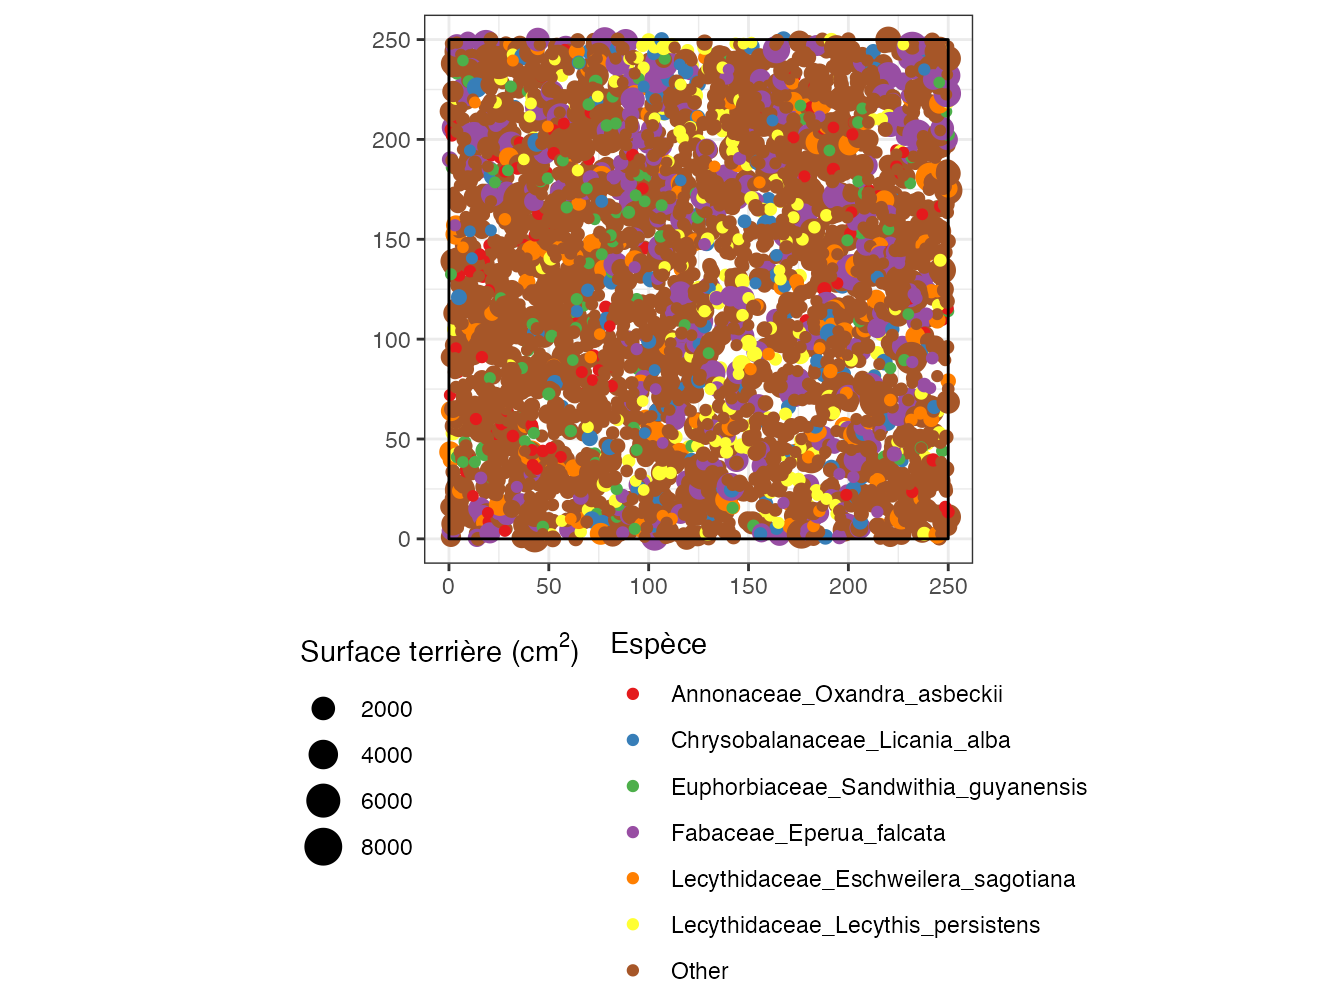
\includegraphics[width=\widthw]{MesuresBD_files/figure-latex/Paracou6MapFig-1} \end{minipage}}\needspace{\ht0+\dp0+2\baselineskip}\definesHSpace\hspace{-\rf}\box0\caption{Carte de la parcelle 6 de Paracou. Les points représentent les arbres. Leur taille est proportionnelle à leur surface terrière. Seules les espèces les plus fréquentes sont identifiées sur la carte.}\label{fig:Paracou6MapFig}
\end{figure}

\normalsize

Le code R pour réaliser la figure est le suivant:

\scriptsize

\begin{Shaded}
\begin{Highlighting}[]
\FunctionTok{library}\NormalTok{(}\StringTok{"divent"}\NormalTok{)}
\NormalTok{paracou\_6\_wmppp }\SpecialCharTok{\%\textgreater{}\%} 
\FunctionTok{autoplot}\NormalTok{(}
  \AttributeTok{labelSize =} \FunctionTok{expression}\NormalTok{(}\FunctionTok{paste}\NormalTok{(}\StringTok{"Surface terrière ("}\NormalTok{, cm}\SpecialCharTok{\^{}}\DecValTok{2}\NormalTok{, }\StringTok{")"}\NormalTok{)), }
  \AttributeTok{labelColor =} \StringTok{"Espèce"}
\NormalTok{) }\SpecialCharTok{+}
\FunctionTok{theme}\NormalTok{(}\AttributeTok{legend.position =} \StringTok{"bottom"}\NormalTok{, }\AttributeTok{legend.direction =} \StringTok{"vertical"}\NormalTok{, }\AttributeTok{legend.margin=}\FunctionTok{margin}\NormalTok{())}
\end{Highlighting}
\end{Shaded}

\normalsize

\hypertarget{notations}{%
\chapter*{Notations}\label{notations}}
\addcontentsline{toc}{chapter}{Notations}

Les notations mathématiques peuvent différer de celles de la littérature citée pour l'homogénéité de ce document.

Les matrices sont notées en caractères gras et majuscules: \(\mathbf{X}\).
Les éléments de la matrice \(\mathbf{X}\) sont notés \(x_{i,j}\).

Les vecteurs sont notés en gras minuscule: \(\mathbf{p}\).
Les nombres sont notés en minuscules, \(n\), et les variables aléatoires en majuscules: \(N\).
Les valeurs maximales des énumérations font exception: elles sont notées en majuscules pour les distinguer des indices: \(\sum_{s=1}^{S}{p_s}=1\).

Le produit matriciel de \(\mathbf{X}\) et \(\mathbf{Y}\) est noté \(\mathbf{X}\mathbf{Y}\). Dans les scripts R, l'opérateur est \texttt{\%*\%}.
Le produit de Hadamard (terme à terme) est noté \(\mathbf{X}\circ\mathbf{Y}\) (opérateur \texttt{*} dans R).
De même \(\mathbf{X}^n\) indique la puissance \(n\) au sens du produit matriciel d'une matrice carrée (opérateur \texttt{\%\^{}\%} du package \emph{expm}), alors que \(\mathbf{X}^{\circ n}\) est la matrice dont chaque terme est celui de \(\mathbf{X}\) à la puissance \(n\) (opérateur \texttt{\^{}} de R).
La matrice transposée de \(\mathbf{X}\) est notée \(\mathbf{X'}\).

Les notations sont les suivantes:

\noindent \({\mathbf 1}(\cdot)\): la fonction indicatrice, qui vaut 1 si la condition dans la parenthèse est vraie, 0 sinon.

\noindent \(\mathbf{1}_s\): le vecteur de longueur \(s\) composé uniquement de 1. \(\mathbf{1}_s\mathbf{1}_s'=\mathbf{J}_s\) où \(\mathbf{J}_s\) est la matrice carré de taille \(s\) ne contenant que des 1.

\noindent \(A\): l'aire d'étude, et, selon le contexte, sa surface.

\noindent \(\alpha_\nu\): la probabilité moyenne des espèces représentées par \(\nu\) individus.

\noindent \(C\): le taux de couverture de l'échantillon, c'est-à-dire la probabilité qu'un individu de la communauté appartienne à une des espèces échantillonnées.
\(C^{n}\) est le taux de couverture correspondant à un échantillon de taille \(n\).

\noindent \(^{q}\!D\): la diversité vraie (nombre de Hill pour les diversités \(\alpha\) et \(\gamma\)), nombre équivalent de communautés pour la diversité \(\beta\).
\(^{q}_{i}\!D_{\alpha}\) est la diversité \(\alpha\) mesurée dans la communauté \(i\).
\(^{q}\!\bar{D}\left(T\right)\) est la diversité phylogénétique.

\noindent \(\boldsymbol{\Delta}\): la matrice de dissimilarité dont les éléments sont \(\delta_{s,t}\), la dissimilarité entre l'espèce \(s\) et l'espèce \(t\).

\noindent \({\mathbb E}\left(X\right)\): l'espérance de la variable aléatoire \(X\).

\noindent \(^{q}\!H\): l'entropie de Tsallis (ou HCDT).
\(^{q}_{i}\!H_{\alpha}\) est l'entropie \(\alpha\) mesurée dans la communauté \(i\).
Si nécessaire, le vecteur des probabilités servant au calcul est précisé sous la forme \(^{q}\!H(\mathbf{p})\).
\(^{q}\!\bar{H}(T)\) est l'entropie phylogénétique.

\noindent \(I\): le nombre de communautés qui constituent une partition de la méta-communauté dans le cadre de la décomposition de la diversité.
Les communautés sont indexées par \(i\).

\noindent \(I(p_s)\): l'information apportée par l'observation d'un évènement de probabilité \(p_s\).
\(I(q_s,p_s)\) est le gain d'information apporté par l'expérience (\(q_s\) est observé) par rapport aux probabilités \(p_s\) attendues.

\noindent \(\mathbf{I}_s\): la matrice identité de rang \(s\): matrice carrée de taille \(s\times s\) dont la diagonale ne comporte que des 1 et les autres élements sont nuls.

\noindent \(N\): le nombre (aléatoire) d'individus se trouvant dans l'aire d'étude.
\(N_s\) est la même variable aléatoire, mais restreinte aux individus de l'espèce \(s\).

\noindent \(n\): le nombre d'individus échantillonnés.
\(n_{s,i}\) est le nombre d'individus de l'espèce \(s\) dans la communauté \(i\).
Les effectifs totaux sont \(n_{s+}\) (pour l'espèce \(s\)), \(n_{+i}\) pour la communauté \(i\) et \(n\) le total général.
S'il n'y a qu'une communauté, le nombre d'individus par espèce est \(n_s\).

\noindent \(p_s\): la probabilité qu'un individu tiré au hasard appartienne à l'espèce \(s\).
Son estimateur, \({\hat{p}}_s\) est la fréquence observée.
\(p_{s|i}\) est la même probabilité dans la communauté \(i\).

\noindent \(\mathbf{p}=\left( p_1, p_2, \dots, p_s, \dots, p_S \right)\): le vecteur décrivant la distribution des probabilités \(p_s\), appelé simplexe en référence à sa représentation dans l'espace à \(S\) dimensions.

\noindent \({\pi}_{\nu}\): la probabilité qu'une espèce choisie au hasard soit représentée par \(\nu\) individus, \(\sum^n_{\nu=1}{{\pi}_{\nu}}\)=1.
Si l'espèce est choisie explicitement, la probabilité est notée \({\pi}_{n_s}\).

\noindent \(^{q}\!R\): l'entropie de Rényi d'ordre \(q\).

\noindent \(S\): le nombre d'espèces, considéré comme une variable aléatoire, estimé par \(\hat{S}\).

\noindent \(S_{\nu}(n)\): le nombre d'espèces, considéré comme une variable aléatoire, observées \(\nu\) fois dans un échantillon de \(n\) individus.
L'indice est le nombre de fois où l'espèce est détectée: par exemple \(S_{1}\) ou \(S_{\ne 0}\).
La surface \(A\) peut remplacer le nombre d'individus \(n\): \(S_{0}(A)\) est le nombre d'espèces non rencontrées dans la surface \(A\).
Pour alléger les notations, s'il n'y a pas d'ambiguïté, l'indice est omis pour les espèces présentes: \(S_{\ne 0}(A)\) est noté \(S^{A}\).

\noindent \(s_{\nu}(n)\): le nombre d'espèces observées, avec les mêmes notations que ci-dessus.
\(s_{\nu}(n)\) peut être considéré comme une réalisation de \(S_{\nu}(n)\).

\noindent \(t^{n}_{1-\alpha/2}\): le quantile d'une loi de Student à \(n\) degrés de liberté au seuil de risque \(\alpha\), classiquement 1,96 pour \(n\) grand et \(\alpha=5\%\).

\noindent \(\mathbf{Z}\): la matrice de similarité entre espèces dont les éléments sont \(z_{s,t}\), la similarité entre l'espèce \(s\) et l'espèce \(t\).

\noindent \(\mathrm{\Gamma}(\cdot)\): la fonction gamma.

\noindent \(\mathrm{\Psi}(\cdot)\): la fonction digamma.

\noindent \(\binom{n}{k}\): le nombre de combinaisons de \(k\) éléments parmi \(n\): \[\binom{n}{k}=\frac{n!}{k!\,(n-k)!}\].

\mainmatter

\hypertarget{part-notions}{%
\part{Notions}\label{part-notions}}

\hypertarget{chap-Notions}{%
\chapter{Notions de Diversité}\label{chap-Notions}}

\hypertarget{composantes}{%
\section{Composantes}\label{composantes}}



\scriptsize

\begin{SCfigure}

{\centering 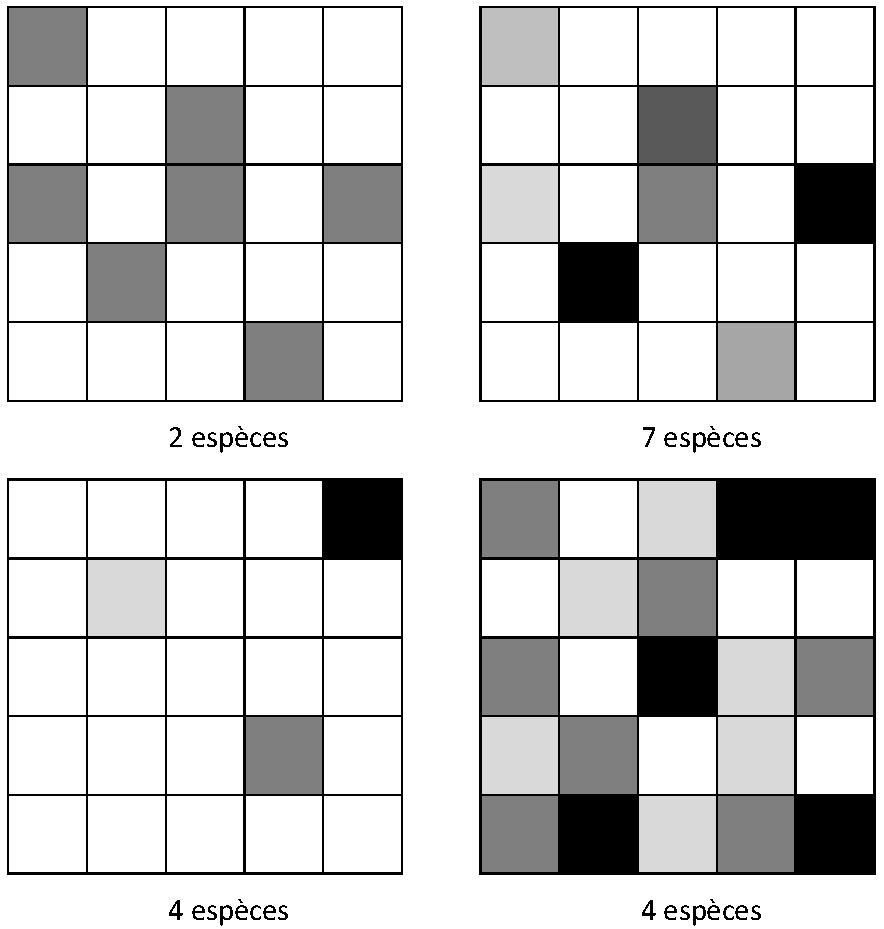
\includegraphics[width=0.6\linewidth]{images/Composantes} 

}

\caption{Importance de la richesse (en haut) et de l'équitabilité (en bas) pour la définition de la diversité. Ligne du haut: toutes choses égales par ailleurs, une communauté de 7 espèces semble plus diverse qu'une communauté de 2 espèces. Ligne du bas: à richesse égale, une communauté moins équitable (à gauche) semble moins diverse. Colonne de gauche: une communauté moins riche (en haut) peut sembler plus diverse si elle est plus équitable. Colonne de droite: idem pour la communauté du bas.}\label{fig:Composantes}
\end{SCfigure}

\normalsize

Une communauté comprenant beaucoup d'espèces mais avec une espèce dominante n'est pas perçue intuitivement comme plus diverse qu'une communauté avec moins d'espèces, mais dont les effectifs sont proches (figure \ref{fig:Composantes}, colonne de gauche).
La prise en compte de deux composantes de la diversité, appelées richesse et équitabilité, est nécessaire \autocite{Whittaker1965}.

\hypertarget{richesse}{%
\subsection{Richesse}\label{richesse}}

La richesse \autocite[terme introduit par][]{Mcintosh1967} est le nombre (ou une fonction croissante du nombre) de classes différentes présentes dans le système étudié, par exemple le nombre d'espèces d'arbres dans une forêt.

Un certain nombre d'hypothèses sont assumées plus ou moins explicitement:

\begin{itemize}
\tightlist
\item
  Les classes sont bien connues: compter le nombre d'espèces a peu de sens si la taxonomie n'est pas bien établie.
  C'est parfois une difficulté majeure quand on travaille sur les micro-organismes;
\item
  Les classes sont équidistantes: la richesse augmente d'une unité quand on rajoute une espèce, que cette espèce soit proche des précédentes ou extrêmement originale.
\end{itemize}

L'indice de richesse le plus simple et le plus utilisé est tout simplement le nombre d'espèces \(S\).

\hypertarget{uxe9quitabilituxe9}{%
\subsection{Équitabilité}\label{uxe9quitabilituxe9}}

La régularité de la distribution des espèces (équitabilité en Français, \emph{evenness} ou \emph{equitability} en anglais) est un élément important de la diversité.
Une espèce représentée abondamment ou par un seul individu n'apporte pas la même contribution à l'écosystème.
Sur la figure \ref{fig:Composantes}, la ligne du bas présente deux communautés de 4 espèces, mais celle de droite est beaucoup plus équitable de celle de gauche et semble intuitivement plus diverse.
À nombre d'espèces égal, la présence d'espèces très dominantes entraîne mathématiquement la rareté de certaines autres: on comprend donc assez intuitivement que le maximum de diversité sera atteint quand les espèces auront une répartition très régulière.

Un indice d'équitabilité est indépendant du nombre d'espèces (donc de la richesse).

La plupart des mesures de diversité courantes, comme celle de Simpson ou de Shannon, évaluent à la fois la richesse et l'équitabilité.

\hypertarget{disparituxe9}{%
\subsection{Disparité}\label{disparituxe9}}

Les mesures classiques de la diversité, dites mesures de diversité neutre (\emph{species-neutral diversity}) ou taxonomique ne prennent pas en compte une quelconque distance entre classes.
Pourtant, deux espèces du même genre sont de toute évidence plus proches que deux espèces de familles différentes.
Les mesures de diversité non neutres (chapitre \ref{chap-cadrephyfonc}) prennent en compte cette notion, qui nécessite quelques définitions supplémentaires \autocite{Mouillot2005,Ricotta2007}.

La mesure de la différence entre deux classes est souvent une distance, mais parfois une mesure qui n'a pas toutes les propriétés d'une distance: une dissimilarité.
Les mesures de \emph{divergence} \autocite{Pavoine2011} sont construites à partir de la dissimilarité entre les classes, avec ou sans pondération par la fréquence.

Si la divergence entre espèces est une distance évolutive comme l'âge du plus récent ancêtre commun, la diversité sera dite phylogénétique.
Si c'est une distance fonctionnelle, définie par exemple dans l'espace des traits fonctionnels, la diversité sera dite fonctionnelle.

La disparité \autocite{Runnegar1987}, divergence moyenne entre deux espèces (indépendamment des fréquences), ou de façon équivalente la longueur totale des branches d'un arbre phylogénétique, est la composante qui décrit à quel point les espèces sont différentes les unes des autres.

Les mesures de \emph{régularité} décrivent la façon dont les espèces occupent l'espace des niches (régularité fonctionnelle) ou la régularité dans le temps et entre les clades des évènements de spéciation représentés par un arbre phylogénétique.
Ce concept complète celui d'équitabilité dans les mesures classiques: la diversité augmente avec la richesse, la divergence entre espèces, et la régularité (qui se réduit à l'équitabilité quand toutes les espèces sont également divergentes entre elles).

\hypertarget{agruxe9gation}{%
\subsection{Agrégation}\label{agruxe9gation}}

À partir d'une large revue de la littérature dans plusieurs disciplines scientifiques s'intéressant à la diversité (au-delà de la biodiversité), \textcite{Stirling2007} estime que les trois composantes, qu'il nomme \emph{variété} (richesse), \emph{équilibre} (équitabilité) et \emph{disparité}, recouvrent tous les aspects de la diversité.

Stirling définit la propriété d'\emph{agrégation} comme la capacité d'une mesure de diversité à combiner explicitement les trois composantes précédentes.
Cela ne signifie pas que les composantes contribuent indépendamment les unes des autres à la diversité \autocite{Jost2010}.

\hypertarget{niveaux-de-luxe9tude}{%
\section{Niveaux de l'étude}\label{niveaux-de-luxe9tude}}

La diversité est classiquement estimée à plusieurs niveaux emboîtés, nommés \(\alpha\), \(\beta\) et \(\gamma\) par \textcite[page 320]{Whittaker1960} qui a nommé \(\alpha\) la diversité locale qu'il mesurait avec l'indice \(\alpha\) de Fisher (voir le chapitre \ref{chap-Fisher}) et a utilisé les lettres suivantes selon ses besoins.

\hypertarget{diversituxe9-alpha-beta-et-gamma}{%
\subsection{\texorpdfstring{Diversité \(\alpha\), \(\beta\) et \(\gamma\)}{Diversité \textbackslash alpha, \textbackslash beta et \textbackslash gamma}}\label{diversituxe9-alpha-beta-et-gamma}}

La diversité \(\alpha\) est la diversité locale, mesurée à l'intérieur d'un système délimité.
Plus précisément, il s'agit de la diversité dans un habitat uniforme de taille fixe.



\scriptsize

\begin{SCfigure}

{\centering 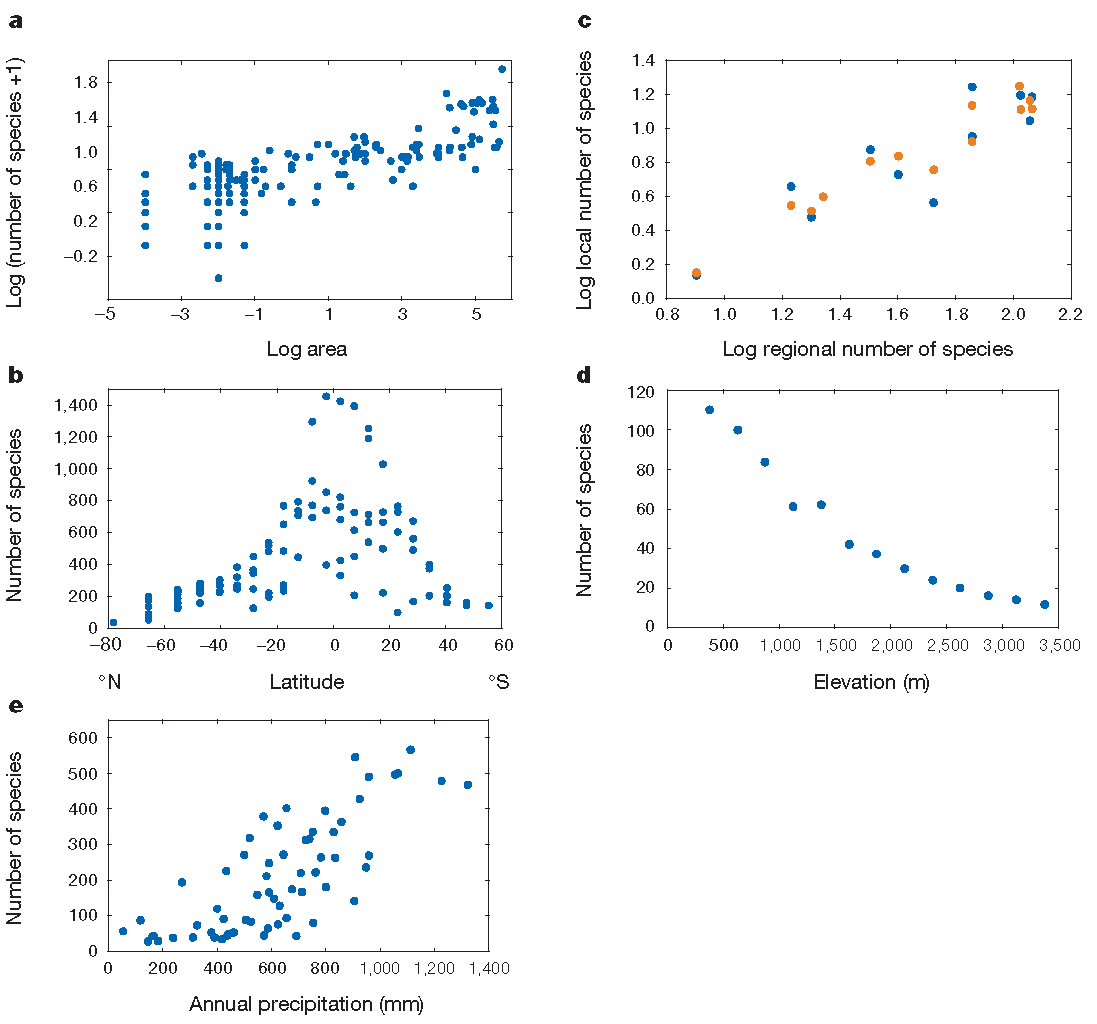
\includegraphics[width=1\linewidth]{images/Gaston2000} 

}

\caption{Patrons de biodiversité. (a) Le nombre d'espèces de vers de terre augmente en fonction de la surface échantillonnée, de 100 m² à plus de 500000 km² selon la relation d'Arrhenius). (b) Nombre d'espèces d'oiseaux en fonction de la latitude. (c) Relation entre la richesse régionale et la richesse locale. (d) Nombre d'espèces de chauves-souris en fonction de l'altitude dans une réserve au Pérou. (e) Nombre d'espèces de végétaux ligneux en fonction des précipitations en Afrique du Sud.}\label{fig:Gaston2000}
\end{SCfigure}

\normalsize

De façon générale \autocite{Gaston2000}, la richesse spécifique diminue avec la latitude (la diversité est plus grande dans les zones tropicales, et au sein de celles-ci, quand on se rapproche de l'équateur), voir figure \ref{fig:Gaston2000} \autocite[figure 1]{Gaston2000}.
La tendance est la même pour la diversité génétique intraspécifique \autocite{Miraldo2016}.
La richesse diminue avec l'altitude.
Elle est généralement plus faible sur les îles, où elle décroît avec la distance au continent, source de migrations.

La diversité \(\beta\) mesure à quel point les systèmes locaux sont différents.
Cette définition assez vague a fait l'objet de nombreux débats \autocite{Moreno2010}.

Enfin, la diversité \(\gamma\) est similaire à la diversité \(\alpha\), prise en compte sur l'ensemble du système étudié.
Les diversités \(\alpha\) et \(\gamma\) se mesurent donc de la même façon, mais à différentes échelles.

\hypertarget{duxe9composition}{%
\subsection{Décomposition}\label{duxe9composition}}

\textcite{Whittaker1977} a proposé sans succès une normalisation des échelles d'évaluation de la biodiversité, en introduisant la diversité régionale \(\varepsilon\) (\(\gamma\) étant réservé au paysage et \(\alpha\) à l'habitat) et la diversité \(\delta\) entre les paysages.
Seuls les trois niveaux originaux ont été conservés par la littérature, sans définition stricte des échelles d'observation.

La distinction entre les diversités \(\alpha\) et \(\beta\) dépend de la finesse de la définition de l'habitat.
La distinction de nombreux habitats diminue la diversité \(\alpha\) au profit de la \(\beta\).
Il est donc important de définir une mesure qui ne dépende pas de ce découpage, donc une mesure cumulative (additive ou multiplicative) décrivant la diversité totale, décomposable en la somme ou le produit convenablement pondérés de toutes les diversités \(\alpha\) des habitats (diversité intra) et de la diversité \(\beta\) inter-habitat.

Nous appellerons \emph{communauté} le niveau de découpage concernant la diversité \(\alpha\) et \emph{méta-communauté} le niveau de regroupement pour l'estimation de la diversité \(\gamma\).

\hypertarget{courbes-daccumulation}{%
\section{Courbes d'accumulation}\label{courbes-daccumulation}}



\scriptsize

\begin{SCfigure}

{\centering 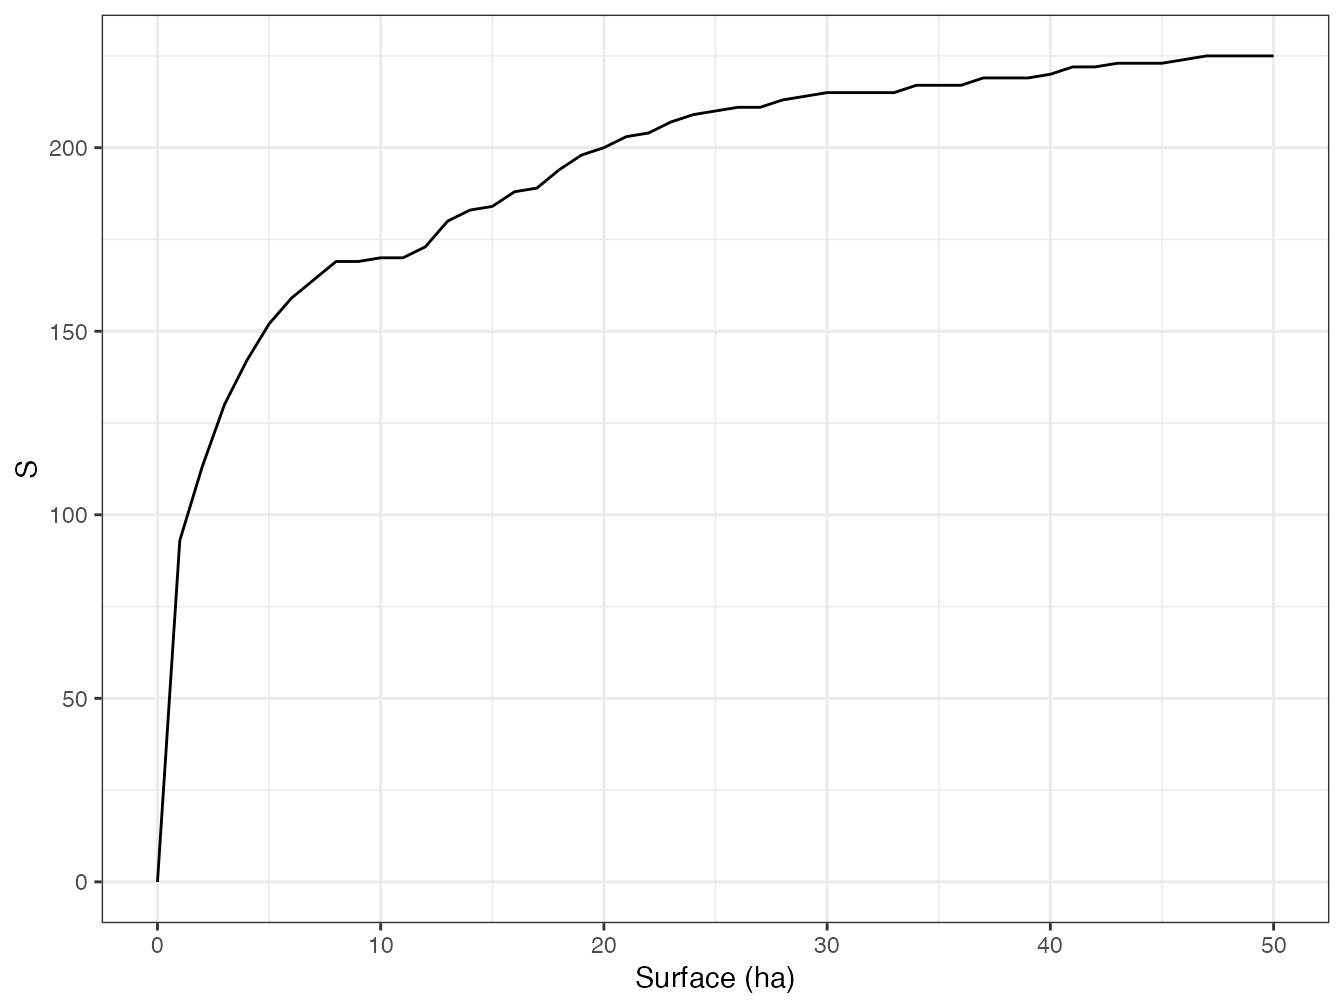
\includegraphics[width=0.8\linewidth]{MesuresBD_files/figure-latex/SACFig-1} 

}

\caption{Courbe d'accumulation des espèces d'arbres du dispositif de Barro Colorado Island. Le nombre d'espèces est cumulé dans l'ordre des carrés d'un hectare du dispositif.}\label{fig:SACFig}
\end{SCfigure}

\normalsize

Evaluer la diversité d'une communauté nécessite en pratique de l'inventorier.
Le nombre d'espèces découvertes en fonction de l'effort d'échantillonnage permet de tracer une courbe d'accumulation (SAC: \emph{Species Acumulation Curve}).
Une courbe de raréfaction (\emph{Rarefaction Curve}) peut être calculée en réduisant par des outils statistiques l'effort d'échantillonnage réel pour obtenir une SAC théorique, libérée des aléas de l'ordre de prise en compte des données.

La figure \ref{fig:SACFig} montre l'accumulation des espèces pour les données de BCI.
Une SAC peut être tracée en fonction de la surface, du nombre d'individus ou du nombres de placettes d'échantillonnage, selon les besoins.

Code R pour réaliser la figure \ref{fig:SACFig}:

\scriptsize

\begin{Shaded}
\begin{Highlighting}[]
\FunctionTok{library}\NormalTok{(}\StringTok{"vegan"}\NormalTok{)}
\FunctionTok{data}\NormalTok{(BCI)}
\CommentTok{\# Chaque parcelle (ligne) cumule ses abondances à la précédente}
\NormalTok{cumul }\OtherTok{\textless{}{-}} \FunctionTok{apply}\NormalTok{(BCI, }\DecValTok{2}\NormalTok{, cumsum)}
\CommentTok{\# Le nombre d\textquotesingle{}espèces de chaque parcelle est cumulé }
\NormalTok{Richesse }\OtherTok{\textless{}{-}} \FunctionTok{apply}\NormalTok{(cumul, }\DecValTok{1}\NormalTok{, }\ControlFlowTok{function}\NormalTok{(x) }\FunctionTok{sum}\NormalTok{(x }\SpecialCharTok{\textgreater{}} \DecValTok{0}\NormalTok{))}
\FunctionTok{ggplot}\NormalTok{(}
  \FunctionTok{data.frame}\NormalTok{(}
    \AttributeTok{A =} \DecValTok{0}\SpecialCharTok{:}\DecValTok{50}\NormalTok{, }
    \AttributeTok{S =} \FunctionTok{c}\NormalTok{(}\DecValTok{0}\NormalTok{, Richesse)}
\NormalTok{  )}
\NormalTok{) }\SpecialCharTok{+}
  \FunctionTok{geom\_line}\NormalTok{(}\FunctionTok{aes}\NormalTok{(}\AttributeTok{x =}\NormalTok{ A, }\AttributeTok{y =}\NormalTok{ S)) }\SpecialCharTok{+}
  \FunctionTok{labs}\NormalTok{(}\AttributeTok{x =} \StringTok{"Surface (ha)"}\NormalTok{)}
\end{Highlighting}
\end{Shaded}

\normalsize

Les courbes d'accumulation peuvent aussi concerner la diversité (voir le chapitre \ref{chap-Accumulation}), mesurée au-delà du nombre d'espèces.

Plus généralement, une courbe aire-espèces (SAR: \emph{Species Area Relationship}) représente le nombre d'espèces observées en fonction de la surface échantillonnée (figure \ref{fig:Williamson2001}).
Il existe plusieurs façons de prendre en compte cette relation \autocite{Scheiner2003}, classables en deux grandes familles \autocite{Dengler2009}:

\begin{itemize}
\tightlist
\item
  Dans une SAR au sens strict, chaque point représente une communauté.
  La question traitée est la relation entre le nombre d'espèces et la taille de chaque communauté, en lien avec des processus écologiques;
\item
  Une courbe d'accumulation (SAC) ne représente que l'effet statistique de l'échantillonnage.
  Pour éviter toute confusion, le terme SAR ne doit pas être utilisé pour décrire une SAC.
\end{itemize}

\hypertarget{diversituxe9-asymptotique}{%
\section{Diversité asymptotique}\label{diversituxe9-asymptotique}}

Augmenter l'effort d'échantillonnage peut permettre d'atteindre un stade où la diversité n'augmente plus: sa valeur est appelée \emph{diversité asymptotique}.
Dans des communautés très diverses comme les forêts tropicales, la diversité asymptotique ne peut en général pas être observée sur le terrain à cause de la variabilité de l'environnement: l'augmentation de la surface inventoriée amène à échantillonner dans des communautés différentes avant d'atteindre la diversité asymptotique de la communauté étudiée.
La diversité asymptotique est donc celle d'une communauté théorique qui n'existe généralement pas.
En d'autres termes, c'est la diversité d'une communauté dont l'inventaire disponible serait un échantillon représentatif.

Evaluer la diversité asymptotique nécessite d'utiliser des estimateurs de diversité, dont la précision dépend de l'exhaustivité de l'échantillonnage.
La diversité peut aussi être estimée pour un effort donné: un hectare de forêt ou 5000 arbres par exemple, ou encore un taux de couverture choisi, qui décrit mieux la qualité de l'échantillonnage.

\hypertarget{le-probluxe8me-de-lespuxe8ce}{%
\section{Le problème de l'espèce}\label{le-probluxe8me-de-lespuxe8ce}}

Évaluer la richesse spécifique suppose que les espèces soient définies clairement, ce qui n'est de toute évidence pas le cas \autocite{Casetta2014}.
Le premier aspect du problème concerne la nature des espèces: réalité naturelle ou seulement représentation simplificatrice.
Une analyse historique et philosophique en est faite par \textcite{Richards2010}.
L'autre aspect, avec des conséquences pratiques plus immédiates, concerne leur délimitation.
\textcite{Mayden1997} recense vingt-deux définitions différentes du concept d'espèce.
\textcite{Wilkins2011} estime qu'il n'y a qu'un seul concept d'espèce mais sept définitions, c'est-à-dire sept façons de les identifier, et vingt-sept variations ou mélanges de ces définitions.

La définition historique est celle de \emph{morphoespèce}, qui classe les espèces selon leurs formes, supposées d'abord immuables.
La définition moderne la plus répandue est celle d'espèce \emph{biologique} \autocite{Dobzhansky1937}: un \enquote{groupe de populations naturelles isolées reproductivement les unes des autres} \autocite{Mayr1942}.
Lorsque les populations d'une espèce sont isolées géographiquement, leur capacité à se reproduire ensemble est toute théorique (et rarement vérifiée expérimentalement).
Des populations allopatriques n'ont pas de flux de gènes réels entre elles et peuvent être considérées comme des espèces distinctes selon la définition d'espèce \emph{phylogénétique}: \enquote{le plus petit groupe identifiable d'individus avec un pattern commun d'ancêtres et de descendants} \autocite{Cracraft1983}.
C'est l'unité génétique détectée par la méthode du coalescent pour la délimitation des espèces \autocite{Sukumaran2017}.
Le nombre d'espèces phylogénétiques est bien supérieur au nombre d'espèces biologiques.
Enfin, \textcite{VanValen1976} définit les espèces par la niche écologique qu'elles occupent (à partir de l'exemple des chênes blancs européens) plutôt que par les flux de gènes (permanents entre les espèces distinctes): la définition \emph{écologique} d'espèce est proche du concept de complexe d'espèces \autocite[ensemble d'espèces voisines échangeant des gènes,][]{Pernes1984}.

Le choix de la définition modifie considérablement sur la quantification de la richesse \autocite{Agapow2004}.
Des problèmes méthodologiques s'ajoutent aux problèmes conceptuels \autocite{Hey2001}: la séparation ou le regroupement de plusieurs populations ou morphotypes en un nombre plus ou moins grand d'espèces est un choix qui reflète les connaissances du moment et peut évoluer \autocite{Barberousse2014}.

L'impact du problème de l'espèce sur la mesure de la diversité reste sans solution à ce stade, si ce n'est d'utiliser les mêmes définitions si des communautés différentes doivent être comparées.
L'approche phylogénétique (chapitre \ref{chap-Phyloentropie}) permet de contourner le problème: si deux taxons très semblables apportent à peine plus de diversité qu'un seul taxon, le choix de les distinguer ou non n'est pas critique.

\hypertarget{distribution-de-labondance-des-espuxe8ces-sad}{%
\chapter{Distribution de l'abondance des espèces (SAD)}\label{distribution-de-labondance-des-espuxe8ces-sad}}

La distribution de l'abondance des espèces (SAD: \emph{Species Abundance Distribution}) est la loi statistique qui donne l'abondance attendue de chaque espèce d'une communauté.
Les espèces ne sont pas identifiées individuellement, mais par le nombre d'individus leur appartenant.



\scriptsize

\begin{SCfigure}

{\centering 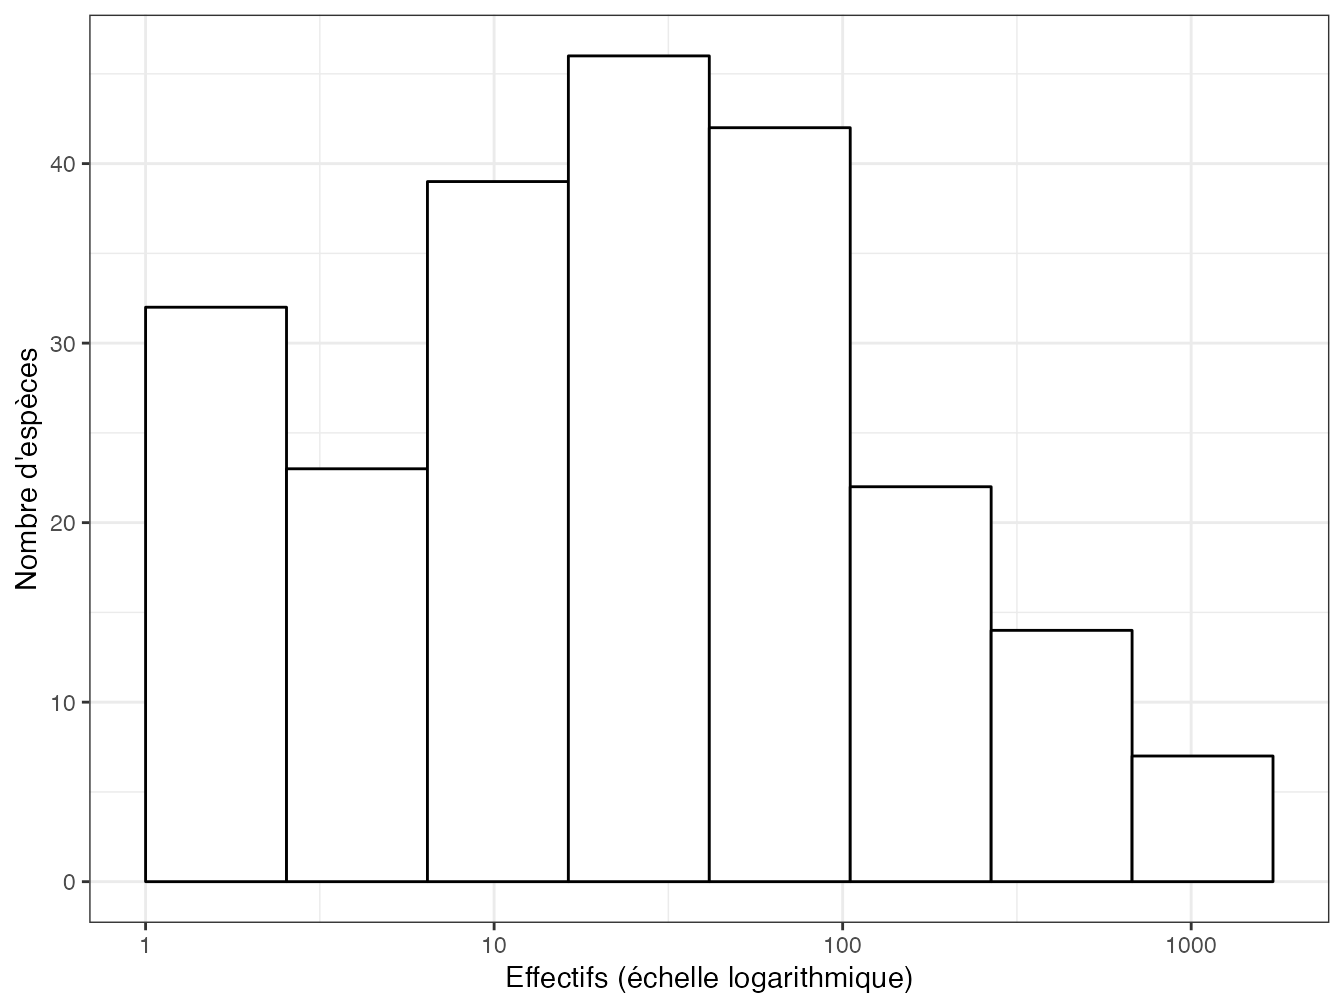
\includegraphics[width=0.8\linewidth]{MesuresBD_files/figure-latex/SADFig-1} 

}

\caption{Histogramme des fréquences (diagramme de Preston) des arbres du dispositif de Barro Colorado Island. En abscisse: le nombre d'arbres de chaque espèce (en logarithme); en ordonnée: le nombre d'espèces.}\label{fig:SADFig}
\end{SCfigure}

\normalsize

Elle peut être représentée sous la forme d'un histogramme des fréquences (diagramme de \textcite{Preston1948}, figure \ref{fig:SADFig}) ou bien d'un diagramme rang-abondance (RAC: \emph{Rank Abundance Curve} ou diagramme de \textcite{Whittaker1965}, figure \ref{fig:RACFig}).
Le RAC est souvent utilisé pour reconnaître des distributions connues.
\textcite{Izsak2012} ont étudié les propriétés des RAC pour les principales SAD.



\scriptsize

\begin{SCfigure}

{\centering 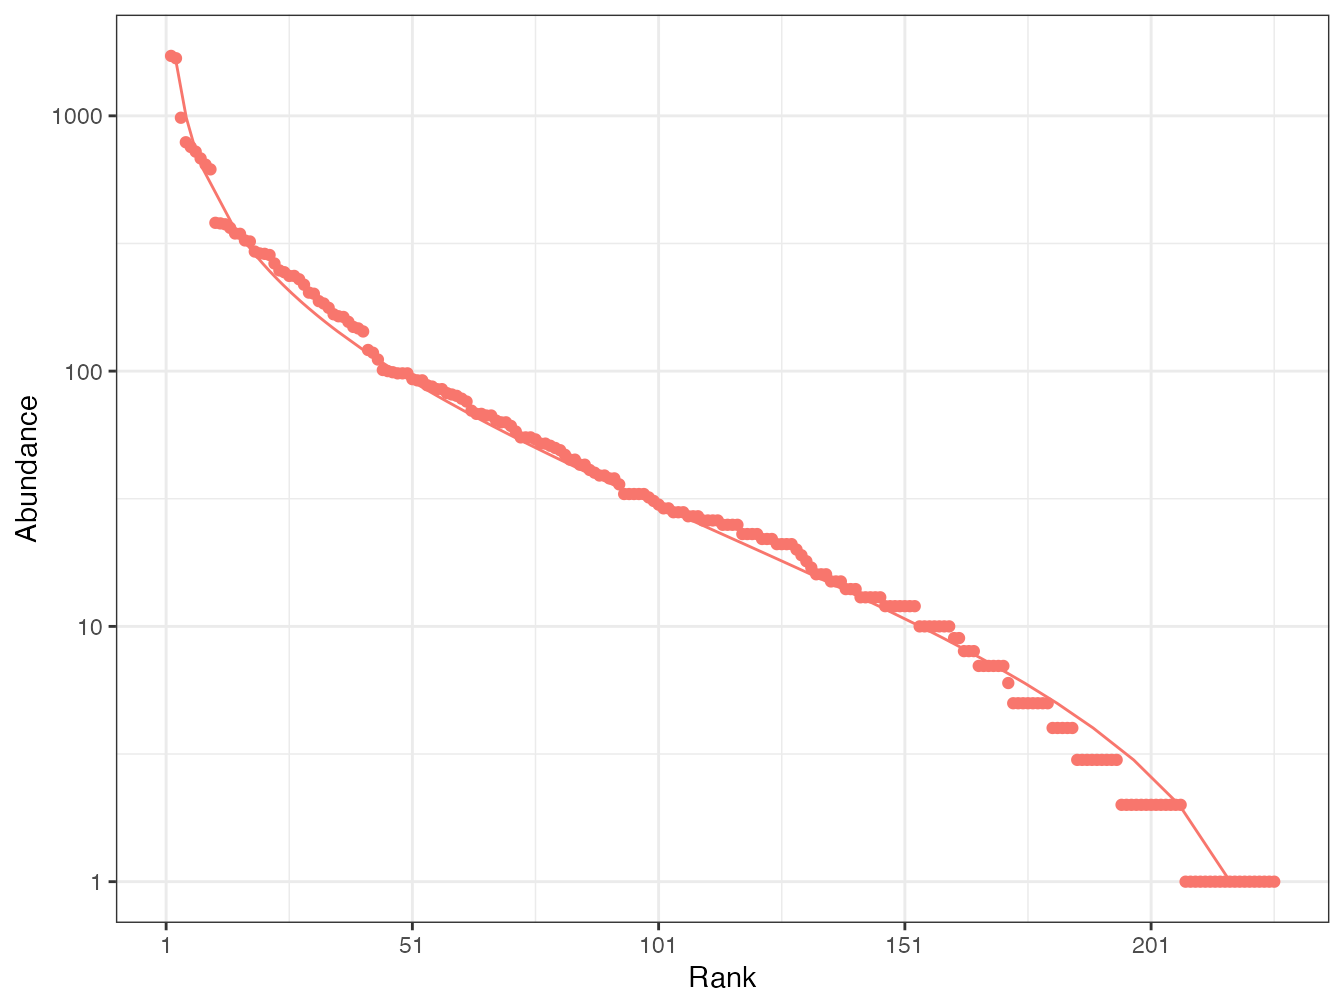
\includegraphics[width=0.8\linewidth]{MesuresBD_files/figure-latex/RACFig-1} 

}

\caption{Diagramme rang-abondance (diagramme de Whittaker) des arbres du dispositif de Barro Colorado Island. Les points sont les données: en abscisse: le rang de l'espèce, à partir de la plus abondante; en ordonnée: l'abondance de l'espèce. La courbe est l'ajustement d'une distribution log-normale.}\label{fig:RACFig}
\end{SCfigure}

\normalsize

Code de la figure \ref{fig:SADFig}:

\scriptsize

\begin{Shaded}
\begin{Highlighting}[]
\NormalTok{BCI\_abd }\OtherTok{\textless{}{-}} \FunctionTok{sort}\NormalTok{(}\FunctionTok{colSums}\NormalTok{(BCI), }\AttributeTok{decreasing =} \ConstantTok{TRUE}\NormalTok{)}
\FunctionTok{ggplot}\NormalTok{(}\FunctionTok{data.frame}\NormalTok{(BCI\_abd), }\FunctionTok{aes}\NormalTok{(BCI\_abd)) }\SpecialCharTok{+} 
  \FunctionTok{geom\_histogram}\NormalTok{(}
    \AttributeTok{bins =} \FunctionTok{nclass.Sturges}\NormalTok{(}\FunctionTok{log}\NormalTok{(BCI\_abd)), }
    \AttributeTok{color =} \StringTok{"black"}\NormalTok{, }
    \AttributeTok{fill =} \StringTok{"white"}\NormalTok{,}
    \AttributeTok{boundary =} \DecValTok{0}
\NormalTok{  ) }\SpecialCharTok{+}
  \FunctionTok{scale\_x\_log10}\NormalTok{() }\SpecialCharTok{+}
  \FunctionTok{labs}\NormalTok{(}
    \AttributeTok{x =} \StringTok{"Effectifs (échelle logarithmique)"}\NormalTok{, }
    \AttributeTok{y =} \StringTok{"Nombre d\textquotesingle{}espèces"}
\NormalTok{  )}
\end{Highlighting}
\end{Shaded}

\normalsize

Code de la figure \ref{fig:RACFig}:

\scriptsize

\begin{Shaded}
\begin{Highlighting}[]
\FunctionTok{library}\NormalTok{(}\StringTok{"divent"}\NormalTok{)}
\NormalTok{BCI\_abd }\SpecialCharTok{\%\textgreater{}\%} 
  \FunctionTok{as\_abundances}\NormalTok{() }\SpecialCharTok{\%\textgreater{}\%} 
  \FunctionTok{autoplot}\NormalTok{(}\AttributeTok{fit\_rac =} \ConstantTok{TRUE}\NormalTok{, }\AttributeTok{distribution =} \StringTok{"lnorm"}\NormalTok{)}
\end{Highlighting}
\end{Shaded}

\normalsize

Les SAD sont traitées en détail par \textcite{Magurran1988} ou \textcite{McGill2007}.
Les principales distributions, nécessaires à la compréhension de la suite sont présentées ici:

\begin{itemize}
\tightlist
\item
  La distribution en log-séries de \textcite{Fisher1943};
\item
  La distribution géométrique \autocite{Motomura1932,Whittaker1972};
\item
  La distribution log-normale \autocite{Preston1948};
\item
  Le modèle Broken Stick \autocite{MacArthur1957}.
\end{itemize}

Formellement, la distribution des probabilités des espèces, notées \(p_s\), est à établir.

\hypertarget{la-distribution-en-log-suxe9ries}{%
\subsection{La distribution en log-séries}\label{la-distribution-en-log-suxe9ries}}

Cette distribution est traitée en détail dans le chapitre \ref{chap-Fisher}.

Le nombre d'espèces est lié au nombre d'individus par la relation \({\mathbb E}(S^n) = \alpha \ln(1 + n / \alpha)\) où \(S^n\) indique le nombre d'espèces observées dans un échantillon de \(n\) individus.
\(\alpha\) est le paramètre qui fixe la pente de la partie linéaire de la relation, valide dès que \(n \gg \alpha\), où le nombre d'espèces \(S^n\) augmente proportionnellement au logarithme du nombre d'individus \(\ln(n)\).

La distribution a été obtenue à partir d'inventaires de communautés de papillons en Malaisie et en Angleterre.
Le modèle est tombé en désuétude faute de confirmation empirique à l'échelle de la communauté, avant d'être remis en valeur par la théorie neutre \autocite{Hubbell2001} dans lequel la distribution de la \emph{méta-communauté} est en log-séries.

\hypertarget{la-distribution-broken-stick}{%
\subsection{La distribution Broken Stick}\label{la-distribution-broken-stick}}

Si les espèces se partagent les ressources ou l'espace des niches, représentées par un bâton, par un processus de cassure aléatoire et simultanée (précisément, les \(S-1\) cassures du bâton sont distribuées uniformément sur sa longueur) et que leur abondance est proportionnelle à la quantité de ressources ou d'espace de niche obtenus, alors leur distribution suit le modèle Broken Stick de \textcite{MacArthur1957}.

Parmi les distributions classiques, c'est la plus équitable: la distribution uniforme des probabilités (\(p_s = 1 / S\) pour tout \(s\)) n'est jamais approchée.

Elle est peu observée empiriquement.

\hypertarget{la-distribution-log-normale}{%
\subsection{La distribution log-normale}\label{la-distribution-log-normale}}

Dans une distribution log-normale, le logarithme des probabilités des espèces (notées \(p_s\) pour l'espèce \(s\)) suit une loi normale.
L'écart-type \(\sigma\) de cette distribution règle l'équitabilité de la distribution.
Son espérance est obtenue à partir du nombre d'espèces et de \(\sigma\), pour que la somme des probabilités égale 1.

\textcite{May1975} explique cette distribution par le théorème de la limite centrale: la variable aléatoire valant 1 si un individu est de l'espèce \(s\) et 0 sinon est le produit de nombreuses variables de loi inconnues valant 1 en cas de succès (germination d'une graine, survie à de nombreux évènements\ldots).
Le logarithme de ce produit est une somme de variables aléatoire dont la loi est forcément normale par application du théorème de la limite centrale.

La distribution est aussi le résultat d'un algorithme de bâton brisé (\emph{broken stick}) hiérarchique \autocite{Bulmer1974}:

\begin{itemize}
\tightlist
\item
  Si les ressources (représentées par un bâton) sont partagées une première fois aléatoirement, selon une loi quelconque,
\item
  Si chaque bâton obtenu est partagé à nouveau selon le même procédé, et que l'opération est répétée un assez grand nombre de fois,
\item
  Si l'abondance de chaque espèce est proportionnelle aux ressources dont elle dispose,
\item
  Alors la distribution des espèces est log-normale.
\end{itemize}

Ce mécanisme décrit assez bien un mécanisme de partage successif des ressources, par exemple entre groupes d'espèces de plus en plus petits, correspondant à des niches écologiques de plus en plus étroites.

D'autres arguments existent dans la littérature.
Par exemple, \textcite{Engen1996} obtiennent une distribution normale à partir d'un modèle de dynamique des populations.

La distribution log-normale décrit assez bien (mais pas exactement) une communauté locale dans le cadre de la théorie neutre \autocite{Hubbell2001} comme le montre la figure \ref{fig:RACFig}.
Le nombre d'espèces rares est un peu surestimé.
La distribution exacte est donnée par \textcite{Volkov2003}.

\hypertarget{la-distribution-guxe9omuxe9trique}{%
\subsection{La distribution géométrique}\label{la-distribution-guxe9omuxe9trique}}

Si les espèces se partagent les ressources selon un algorithme \emph{broken stick} séquentiel (comme dans la distribution log-normale) mais de proportion fixe \(0<k<1\), alors la distribution obtenue est géométrique.
Les abondances successives sont proportionnelles à \(k, k(1-k), k(1-k)^2, \dots, k(1-k)^s, \dots, k(1-k)^S\).

Ce modèle a été établi par \textcite{Motomura1932} cité par \textcite{May1975}.
Ses propriétés ont été étudiées par \textcite{Whittaker1972}.

C'est la distribution qui traduit l'absence de relation entre la taille de l'échantillon et l'abondance des espèces \autocite{Pueyo2007}: la distribution du logarithme de ses probabilités est uniforme.
En d'autre termes, l'ordre de grandeur de l'abondance d'une espèce est uniformément distribué.

La distribution est observée dans les communautés pionnières \autocite{Bazzaz1975}, peu diverses, ou les communautés microbiennes \autocite{Haegeman2013}.

\hypertarget{synthuxe8se}{%
\subsection{Synthèse}\label{synthuxe8se}}



\scriptsize

\begin{SCfigure}

{\centering 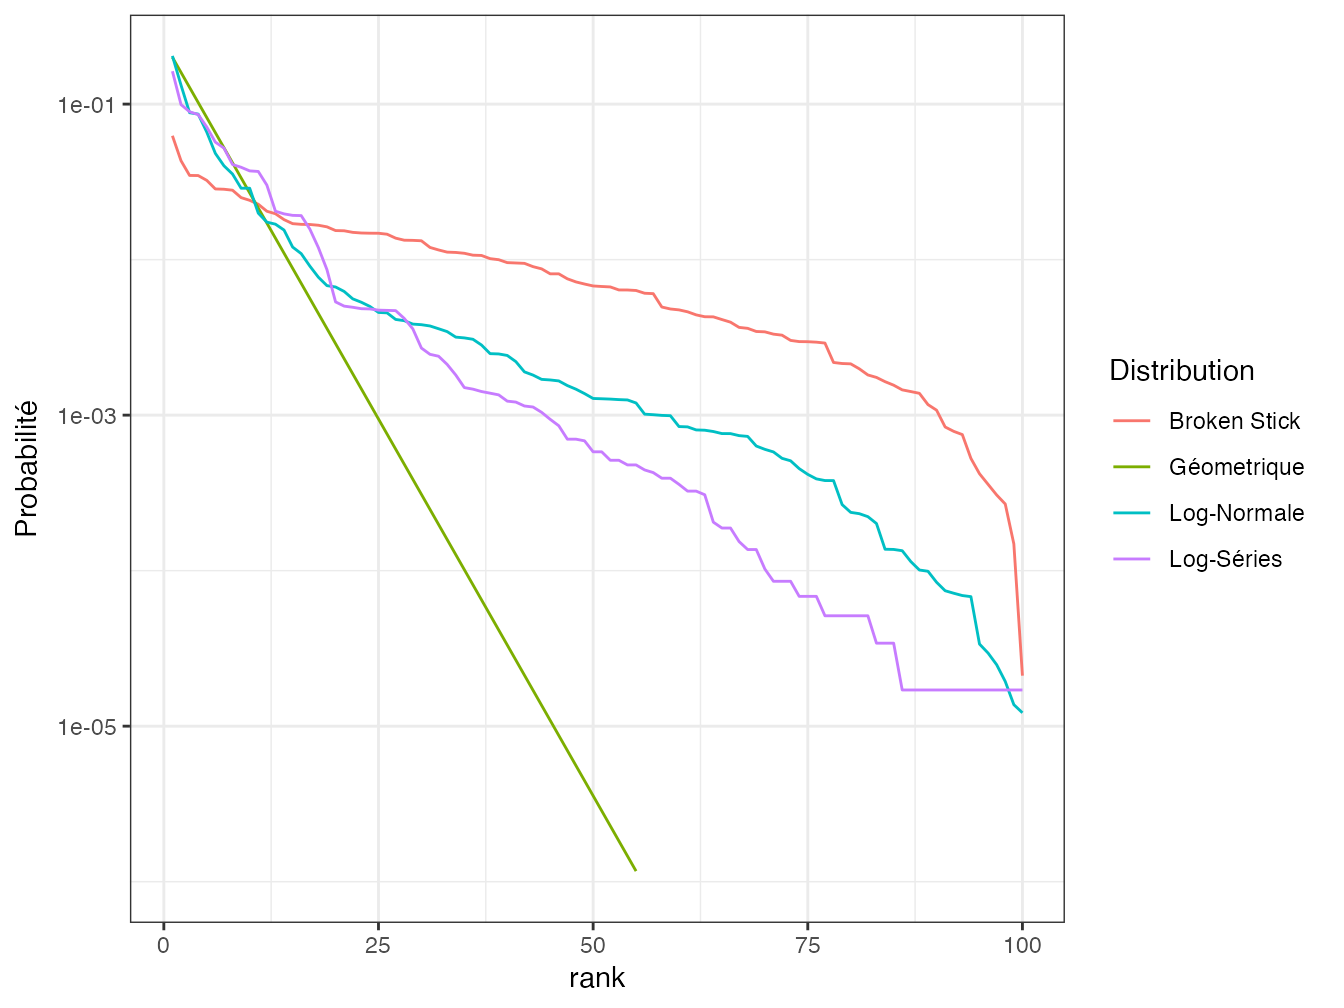
\includegraphics[width=1\linewidth]{MesuresBD_files/figure-latex/DistributionsFig-1} 

}

\caption{Diagramme rang-fréquence des distributions de probabilité classiques. Toutes les distributions sont de 100 espèces. Les probabilités inférieures à \(10^{-6}\) ne sont pas affichées. Les paramètres choisis sont \(\alpha=11\) pour la distribution log-séries, \(k=0,2\) pour la distribution géométrique et \(\sigma=2\) pour la distribution log-normale.}\label{fig:DistributionsFig}
\end{SCfigure}

\normalsize

La figure \ref{fig:DistributionsFig} est inspirée de la figure très connue de \textcite{Magurran1988}.
Elle montre bien une gradation en termes de décroissance de probabilité entre des distributions de même richesse: de la plus équitable (broken stick) à la plus inéquitable (géométrique).
Elle doit être nuancée: la proportion \(k\) de la distribution géométrique fixe la pente de la droite qui la représente sur la figure.
\(k=10\%\) sur la figure: une valeur plus faible diminuerait la pente.
De même, l'écart-type de la distribution log-normale décrit sa dispersion.
Une valeur supérieure augmenterait sa décroissance.

Le code utilisé pour produire la figure \ref{fig:DistributionsFig} est le suivant:

\scriptsize

\begin{Shaded}
\begin{Highlighting}[]
\FunctionTok{library}\NormalTok{(}\StringTok{"divent"}\NormalTok{)}
\CommentTok{\# Tirage d\textquotesingle{}une communauté en log{-}séries}
\NormalTok{size }\OtherTok{\textless{}{-}} \FloatTok{1E5}
\NormalTok{alpha }\OtherTok{\textless{}{-}} \DecValTok{11}
\NormalTok{species\_number }\OtherTok{\textless{}{-}} \SpecialCharTok{{-}}\NormalTok{alpha }\SpecialCharTok{*} \FunctionTok{log}\NormalTok{(alpha }\SpecialCharTok{/}\NormalTok{ (size }\SpecialCharTok{+}\NormalTok{ alpha))}
\NormalTok{abd\_lseries }\OtherTok{\textless{}{-}} \FunctionTok{rlseries}\NormalTok{(species\_number, size, alpha)}
\CommentTok{\# Part des ressources accaparées dans la distribution géométrique}
\NormalTok{prob }\OtherTok{\textless{}{-}} \FloatTok{0.2}
\CommentTok{\# Calcul des probabilités de la distribution géométrique}
\NormalTok{prob\_geom }\OtherTok{\textless{}{-}}\NormalTok{ prob }\SpecialCharTok{/}\NormalTok{ (}\DecValTok{1} \SpecialCharTok{{-}}\NormalTok{ (}\DecValTok{1} \SpecialCharTok{{-}}\NormalTok{ prob)}\SpecialCharTok{\^{}}\NormalTok{species\_number) }\SpecialCharTok{*}\NormalTok{ (}\DecValTok{1} \SpecialCharTok{{-}}\NormalTok{ prob)}\SpecialCharTok{\^{}}\NormalTok{(}\DecValTok{0}\SpecialCharTok{:}\NormalTok{(species\_number }\SpecialCharTok{{-}} \DecValTok{1}\NormalTok{))}
\CommentTok{\# Dispersion de la loi lognormale}
\NormalTok{sd }\OtherTok{\textless{}{-}} \DecValTok{2}
\CommentTok{\# Tirage de S valeurs dans une loi lognormale}
\NormalTok{abd\_lnorm }\OtherTok{\textless{}{-}} \FunctionTok{rlnorm}\NormalTok{(species\_number, }\AttributeTok{meanlog =} \DecValTok{0}\NormalTok{, }\AttributeTok{sdlog =}\NormalTok{ sd)}
\CommentTok{\# Tirage des probabilités de la distribution broken stick}
\NormalTok{prob\_bstick }\OtherTok{\textless{}{-}} \FunctionTok{c}\NormalTok{(cuts }\OtherTok{\textless{}{-}} \FunctionTok{sort}\NormalTok{(stats}\SpecialCharTok{::}\FunctionTok{runif}\NormalTok{(species\_number }\SpecialCharTok{{-}} \DecValTok{1}\NormalTok{)), }\DecValTok{1}\NormalTok{) }\SpecialCharTok{{-}} \FunctionTok{c}\NormalTok{(}\DecValTok{0}\NormalTok{, cuts)}
\CommentTok{\# Graphique}
\FunctionTok{tibble}\NormalTok{(}
  \AttributeTok{rank =} \DecValTok{1}\SpecialCharTok{:}\NormalTok{species\_number,}
  \StringTok{\textasciigrave{}}\AttributeTok{Log{-}Séries}\StringTok{\textasciigrave{}} \OtherTok{=} \FunctionTok{sort}\NormalTok{(abd\_lseries }\SpecialCharTok{/} \FunctionTok{sum}\NormalTok{(abd\_lseries), }\AttributeTok{decreasing =} \ConstantTok{TRUE}\NormalTok{),}
  \StringTok{\textasciigrave{}}\AttributeTok{Géometrique}\StringTok{\textasciigrave{}} \OtherTok{=} \FunctionTok{sort}\NormalTok{(prob\_geom, }\AttributeTok{decreasing =} \ConstantTok{TRUE}\NormalTok{),}
  \StringTok{\textasciigrave{}}\AttributeTok{Log{-}Normale}\StringTok{\textasciigrave{}} \OtherTok{=} \FunctionTok{sort}\NormalTok{(abd\_lnorm }\SpecialCharTok{/} \FunctionTok{sum}\NormalTok{(abd\_lnorm), }\AttributeTok{decreasing =} \ConstantTok{TRUE}\NormalTok{),}
  \StringTok{\textasciigrave{}}\AttributeTok{Broken Stick}\StringTok{\textasciigrave{}} \OtherTok{=} \FunctionTok{sort}\NormalTok{(prob\_bstick, }\AttributeTok{decreasing =} \ConstantTok{TRUE}\NormalTok{)) }\SpecialCharTok{\%\textgreater{}\%} 
  \FunctionTok{pivot\_longer}\NormalTok{(}\AttributeTok{cols =} \SpecialCharTok{{-}}\NormalTok{rank) }\SpecialCharTok{\%\textgreater{}\%} 
  \FunctionTok{ggplot}\NormalTok{() }\SpecialCharTok{+}
    \FunctionTok{geom\_line}\NormalTok{(}\FunctionTok{aes}\NormalTok{(}\AttributeTok{x =}\NormalTok{ rank, }\AttributeTok{y =}\NormalTok{ value, }\AttributeTok{color =}\NormalTok{ name)) }\SpecialCharTok{+}
    \FunctionTok{scale\_y\_log10}\NormalTok{(}\AttributeTok{limits =} \FunctionTok{c}\NormalTok{(}\FloatTok{1E{-}6}\NormalTok{, }\ConstantTok{NA}\NormalTok{)) }\SpecialCharTok{+}
    \FunctionTok{labs}\NormalTok{(}\AttributeTok{y =} \StringTok{"Probabilité"}\NormalTok{, }\AttributeTok{color =} \StringTok{"Distribution"}\NormalTok{)}
\end{Highlighting}
\end{Shaded}

\normalsize

La simulation de ces quatre distributions peut être réalisée par la fonction \texttt{rcommunity()} du package \emph{divent}, où l'argument \texttt{distribution} peut valoir \enquote{bstick}, \enquote{lnorm}, \enquote{geom} ou \enquote{lseries}.
La simulation des communautés autres que log-séries passe par le tirage des probabilités des espèces (le calcul est déterministe dans le cas de la distribution géométrique) puis le tirage d'un nombre d'individus dans une loi multinomiale respectant ces probabilités et l'effectif total.

La fonction \texttt{fit\_rac()} permet d'inférer les paramètres d'une distribution à partir d'un vecteur d'abondance.
La distribution correspondant au modèle estimé peut être affichée sur la figure Rang-Abondance (figure \ref{fig:SADFig}).

Le package \emph{sads} fournit les fonctions classiques de R (densité de probabilité, cumulative, quantile, simulation) pour les distributions utiles en écologie, au-delà de celles présentées ici.
La distribution de Volkov notamment peut être simulée.
Les fonctions \texttt{fitxxx()} complètent la fonction \texttt{fit\_rac()} de \emph{divent}.
Enfin, la fonction \texttt{radfit()} du package \emph{vegan} ajuste aux données en même temps les distributions broken-stick (désignée par \enquote{Null}), géométrique (\enquote{Preemption}) et lognormale, inclut les distributions de Zipf et de Mandelbrot non traitées ici, mais ignore les log-séries.
Les vraisemblances des différents modèles sont comparées pour choisir celui qui s'ajuste le mieux.

Le code suivant montre comment ajuster une distribution log-normale aux données de BCI avec \emph{divent} ou \emph{sads}.

\scriptsize

\begin{Shaded}
\begin{Highlighting}[]
\CommentTok{\# divent}
\FunctionTok{library}\NormalTok{(}\StringTok{"divent"}\NormalTok{)}
\NormalTok{fit\_divent\_lnorm }\OtherTok{\textless{}{-}} \FunctionTok{fit\_rac}\NormalTok{(BCI\_abd, }\AttributeTok{distribution =} \StringTok{"lnorm"}\NormalTok{)}
\CommentTok{\# Affichage des paramètres estimés}
\NormalTok{fit\_divent\_lnorm}\SpecialCharTok{$}\NormalTok{parameters}
\end{Highlighting}
\end{Shaded}

\begin{verbatim}
## # A tibble: 1 x 2
##      mu sigma
##   <dbl> <dbl>
## 1  3.14  1.79
\end{verbatim}

\begin{Shaded}
\begin{Highlighting}[]
\CommentTok{\# sads}
\FunctionTok{library}\NormalTok{(}\StringTok{"sads"}\NormalTok{)}
\CommentTok{\# Estimation. Les données sont tronquées: les espèces observées 0 fois ne sont pas comptées.}
\NormalTok{fit\_sads\_lnorm }\OtherTok{\textless{}{-}} \FunctionTok{fitlnorm}\NormalTok{(BCI\_abd, }\AttributeTok{trunc=}\DecValTok{0}\NormalTok{)}
\NormalTok{fit\_sads\_lnorm}\SpecialCharTok{@}\NormalTok{fullcoef}
\end{Highlighting}
\end{Shaded}

\begin{verbatim}
##  meanlog    sdlog 
## 3.142695 1.787195
\end{verbatim}

\begin{Shaded}
\begin{Highlighting}[]
\CommentTok{\#vegan}
\FunctionTok{library}\NormalTok{(}\StringTok{"vegan"}\NormalTok{)}
\NormalTok{fit\_vegan\_lnorm }\OtherTok{\textless{}{-}} \FunctionTok{radfit}\NormalTok{(BCI\_abd)}
\NormalTok{fit\_vegan\_lnorm}
\end{Highlighting}
\end{Shaded}

\begin{verbatim}
## 
## RAD models, family poisson 
## No. of species 225, total abundance 21457
## 
##            par1      par2     par3    Deviance AIC     
## Null                                  10261.14 11387.97
## Preemption  0.034063                   3788.38  4917.21
## Lognormal   3.3569    1.5738            744.30  1875.13
## Zipf        0.14679  -0.94912          4335.50  5466.33
## Mandelbrot  17.014   -2.0064   15.048   988.02  2120.85
##            BIC     
## Null       11387.97
## Preemption  4920.63
## Lognormal   1881.96
## Zipf        5473.16
## Mandelbrot  2131.10
\end{verbatim}

\normalsize

L'ajustement du modèle de Volkov peut être comparé à celui d'une distribution log-normale.

\scriptsize

\begin{Shaded}
\begin{Highlighting}[]
\CommentTok{\# Ajustement du modèle de Volkov}
\NormalTok{fit\_volkov }\OtherTok{\textless{}{-}} \FunctionTok{fitvolkov}\NormalTok{(BCI\_abd)}
\NormalTok{fit\_volkov}\SpecialCharTok{@}\NormalTok{fullcoef}
\end{Highlighting}
\end{Shaded}

\begin{verbatim}
##        theta            m            J 
## 4.767129e+01 9.238201e-02 2.145700e+04
\end{verbatim}

\normalsize

Graphiquement, l'ajustement est très proche mais la distribution de Volkov prévoit explicitement des effectifs égaux parce qu'entiers.

\scriptsize

\begin{Shaded}
\begin{Highlighting}[]
\CommentTok{\# Comparaison graphique des deux modèles. Log{-}normal en rouge.}
\FunctionTok{plot}\NormalTok{(}\FunctionTok{as\_abundances}\NormalTok{(BCI\_abd), }\AttributeTok{fit\_rac =} \ConstantTok{TRUE}\NormalTok{, }\AttributeTok{distribution=}\StringTok{"lnorm"}\NormalTok{)}
\CommentTok{\# Volkov en vert}
\FunctionTok{lines}\NormalTok{(}
  \FunctionTok{sort}\NormalTok{(}
    \FunctionTok{rvolkov}\NormalTok{(}
      \FunctionTok{length}\NormalTok{(BCI\_abd), }
\NormalTok{      fit\_volkov}\SpecialCharTok{@}\NormalTok{fullcoef[}\DecValTok{1}\NormalTok{], }
\NormalTok{      fit\_volkov}\SpecialCharTok{@}\NormalTok{fullcoef[}\DecValTok{2}\NormalTok{], }
\NormalTok{      fit\_volkov}\SpecialCharTok{@}\NormalTok{fullcoef[}\DecValTok{3}\NormalTok{]}
\NormalTok{    ), }
    \AttributeTok{decreasing=}\ConstantTok{TRUE}
\NormalTok{  ), }
  \AttributeTok{col=}\StringTok{"green"}
\NormalTok{)}
\end{Highlighting}
\end{Shaded}

\begin{center}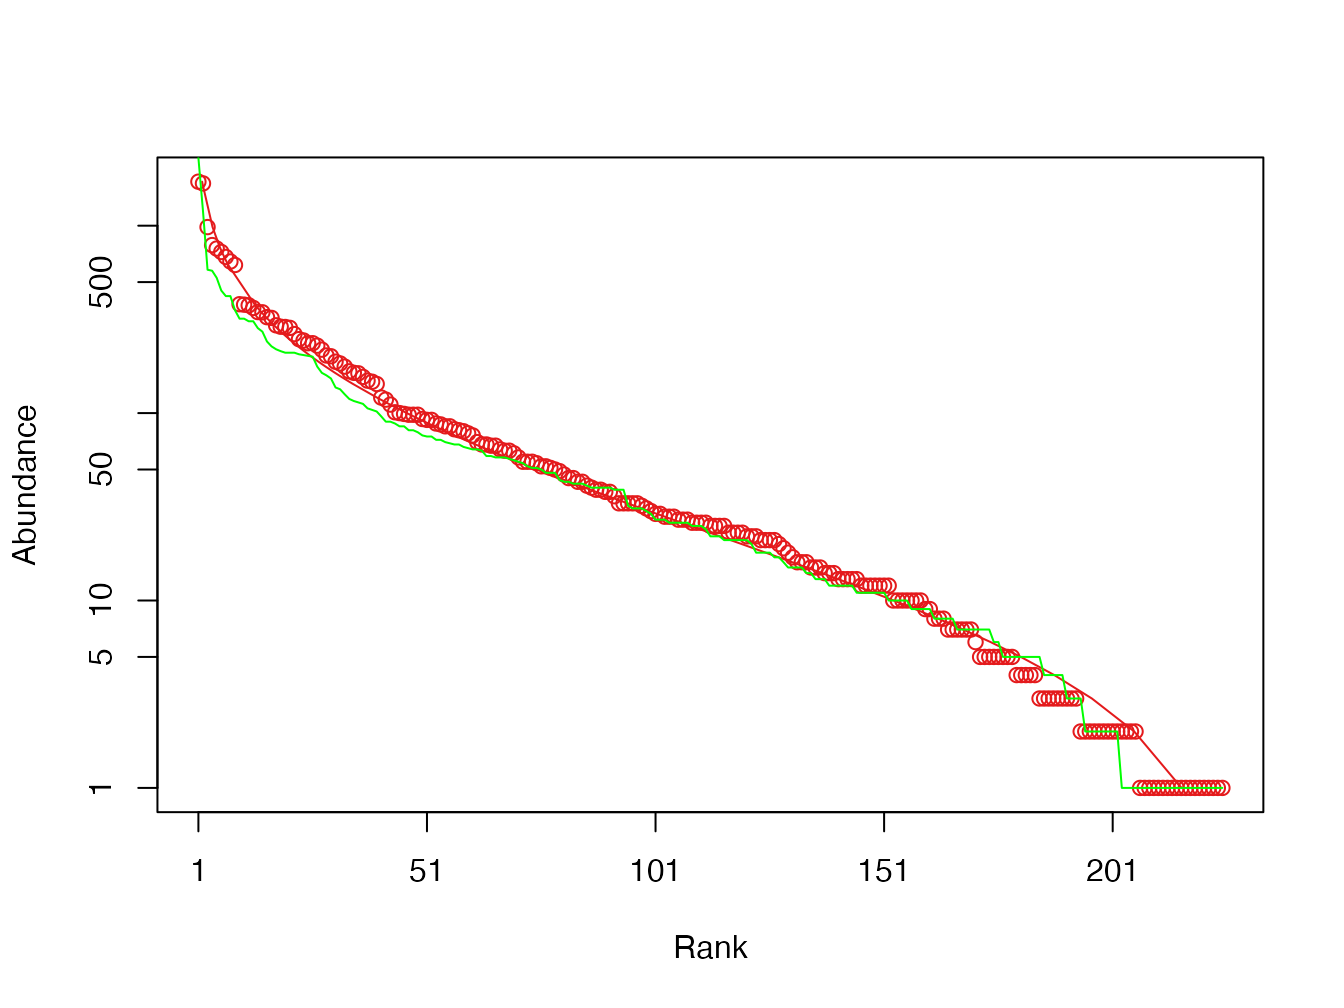
\includegraphics[width=0.8\linewidth]{MesuresBD_files/figure-latex/BCIfit3-1} \end{center}

\normalsize

Les vraisemblances sont proches.

\scriptsize

\begin{Shaded}
\begin{Highlighting}[]
\CommentTok{\# Comparaison des vraisemblances}
\NormalTok{fit\_sads\_lnorm}\SpecialCharTok{@}\NormalTok{min}
\end{Highlighting}
\end{Shaded}

\begin{verbatim}
## [1] 1157.013
\end{verbatim}

\begin{Shaded}
\begin{Highlighting}[]
\NormalTok{fit\_volkov}\SpecialCharTok{@}\NormalTok{min}
\end{Highlighting}
\end{Shaded}

\begin{verbatim}
## [1] 1150.182
\end{verbatim}

\normalsize

Les paramètres du modèle de communauté locale de la théorie neutre sont \(\theta\), le \enquote{nombre fondamental de la biodiversité} égal à deux fois le nombre d'espèces apparaissant par pas de temps dans la méta-communauté, \(m\), le taux de migration, et \(J\), la taille de la communauté locale (qui n'est pas à proprement parler un paramètre mais une statistique décrivant les données).

La différence entre les logarithmes de vraisemblance des deux modèles en faveur du modèle de Volkov, alors que le nombre de paramètres est le même.
L'ajustement est donc meilleur mais la différence est petite et la complexité du modèle et des calculs pour l'estimer ne se justifient pas en général: le modèle de Volkov est très peu utilisé en pratique.


% Bibliography
%%%%%%%%%%%%%%%%%%%%%%%%%%%%%%%%%%%%%%%%%%%%%%%%%%%%%%%%%%

\backmatter
\SmallMargins

\twocolumn
\renewcommand*{\bibfont}{\scriptsize}
\printbibliography
\onecolumn


% Tables (of tables, of figures)
%%%%%%%%%%%%%%%%%%%%%%%%%%%%%%%%%%%%%%%%%%%%%%%%%%%%%%%%%%




% After-body (LaTeX code inclusion)
%%%%%%%%%%%%%%%%%%%%%%%%%%%%%%%%%%%%%%%%%%%%%%%%%%%%%%%%%%




% Back cover
%%%%%%%%%%%%%%%%%%%%%%%%%%%%%%%%%%%%%%%%%%%%%%%%%%%%%%%%%%%

% Even page, small margins, no running head, no page number.
\evenpage
\SmallMargins
\thispagestyle{empty}

\begin{normalsize}

\begin{description}

\selectlanguage{french}
\item[Résumé]
La biodiversité peut être mesurée de nombreuses façons.

La dualité entropie-diversité fournit un cadre clair et rigoureux pour le faire.
L'entropie est la surprise moyenne fournie par les individus d'une communauté.
Le choix de la fonction d'information qui mesure cette surprise à partir des probabilités d'occurence des espèces (ou d'autres catégories) permet de définir les mesures de diversités neutres, fonctionnelles ou phylogénétique présentées ici.
L'entropie est transformée en diversité au sens strict par une fonction croissante (l'exponentielle déformée), ce qui simplifie son interprétation en tant que nombre équivalent d'espèces.

L'entropie phylogénétique généralise les indices de diversité classique, intègre si nécessaire la distance entre espèces, peut être écomposée et corrigée des biais d'estimation.
Sa transformation en diversité au sens strict permet d'interpréter les valeurs sous une forme unique : un nombre équivalent d'espèces et un nombre équivalent de communautés.
La diversité de Leinster et Cobbold généralise à son tour la diversité phylogénétique et permet d'autres définitions de la distance entre espèces.
Le paramétrage des mesures (l'ordre de la diversité) permet de donner plus ou moins d'importance aux espèces rares et de tracer des profils de diversité.

La construction de ce cadre méthodologique est présentée en détail ainsi que plusieurs approches différentes, qui constituent l'état de l'art de la mesure de la biodiversité.
\item[]
.
~\\

\end{description}

\end{normalsize}

\vspace*{\fill}
\centering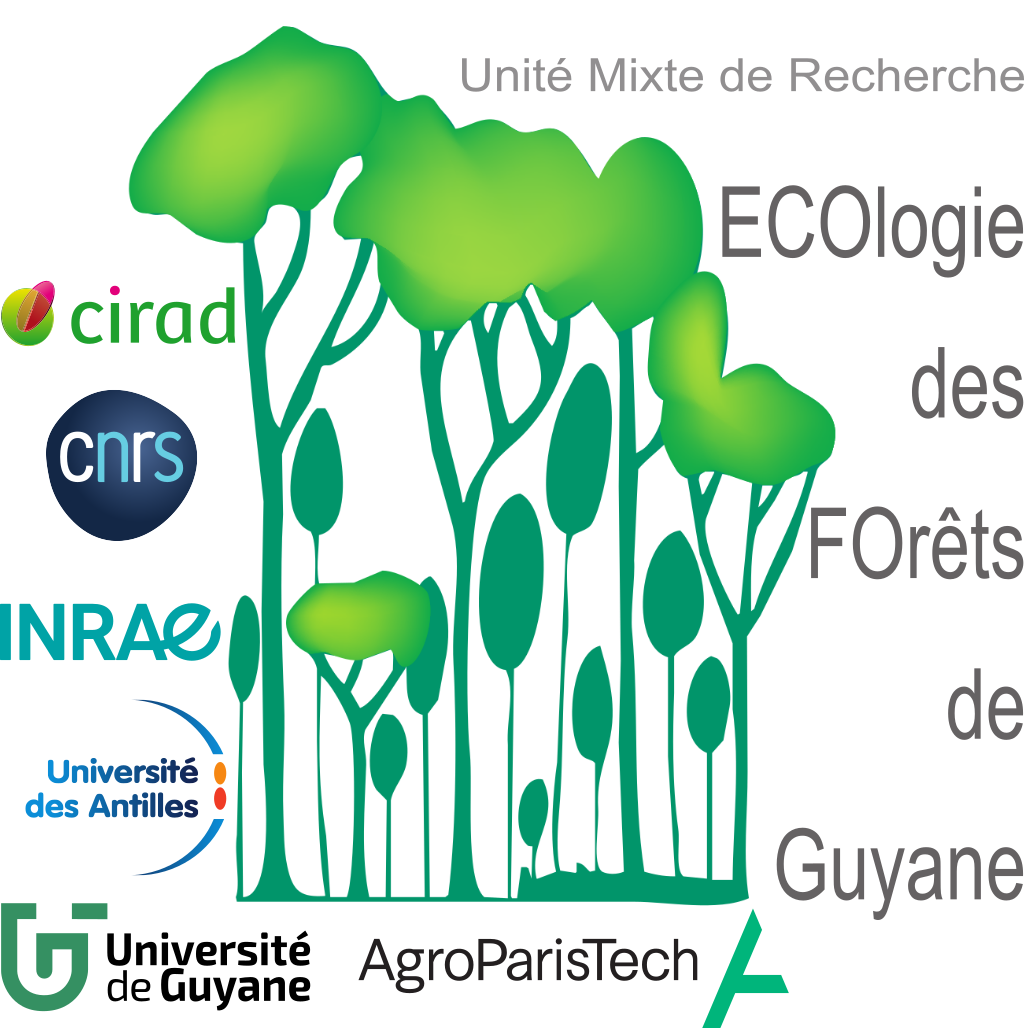
\includegraphics[width=.3\textwidth]{images/logo}

\end{document}
